\documentclass[12pt, final, twoside]{fithesis2}
\usepackage[inner=38mm, outer=27mm, top=37mm, bottom=48mm]{geometry}
\usepackage[utf8]{inputenc}

% searchable and copyable pdf (special characters, accents)
\usepackage{cmap}

% colours and graphics
\usepackage[usenames,dvipsnames,svgnames]{xcolor}

%\usepackage{fontspec}
\usepackage[normalem]{ulem}

\usepackage{subfig}
\usepackage[us,24hr]{datetime}
\newdateformat{mydate}{\THEDAY.\THEMONTH.\THEYEAR}
\newcommand{\verze}{  \scriptsize(v. \mydate\today\ \currenttime)}

% font
\usepackage[T1]{fontenc} % left bottom quote ,,  (,,bla'')
\usepackage{lmodern}
\usepackage{microtype}
\usepackage{indentfirst}
% \usepackage{verbatim}
% \usepackage{moreverb}
\usepackage{setspace} % spacing environment

\usepackage{enumitem}
\setitemize{itemsep=.5ex, topsep=.5ex, parsep=0pt, partopsep=0pt}

\usepackage[ruled,lined]{algorithm2e}
\setlength{\algomargin}{0.5cm}

\newcommand{\argmax}{\operatornamewithlimits{arg\,max}}
\newcommand{\argmin}{\operatornamewithlimits{arg\,min}}


\usepackage[final]{hyperref}

% theorems

\usepackage{framed}


\usepackage{amsmath}
\usepackage{mathtools}  % (in texlive-latex3 package)
\mathtoolsset{showonlyrefs}

%\usepackage[amsmath, amsthm, framed, thmmarks]{ntheorem}
\usepackage[amsmath, amsthm, framed]{ntheorem}

% \usepackage{amsthm}
\usepackage{tikz}
\tikzstyle{thmbox} = [rectangle, rounded corners=10, draw=gray!20, fill=gray!10, inner sep=8pt, inner ysep=1pt]
\newcommand\thmbox[1]{
  % \hspace{-8pt}
  \begin{tikzpicture}
  \node [inner sep=-10pt, inner ysep=-5pt] (box) {
    \begin{tikzpicture}
    \node [thmbox] (box){
      #1
    };
    \end{tikzpicture}
  };
  \end{tikzpicture}
}
\let\theoremframecommand\thmbox

\newcounter{common}
%\numberwithin{common}{section}

\theoremstyle{definition}
\shadecolor{gray!5}
\newshadedtheorem{definition}[common]{Definition}
%\newtheorem{definition}{Definition}
\newtheorem{example}[common]{Example}

\theoremstyle{plain}
\newtheorem{problem}[common]{Problem}
\shadecolor{gray!15}
\newshadedtheorem{theorem}[common]{Theorem}
%\newshadedtheorem{lemma}{Lemma}
%\newtheorem{theorem}{Theorem}
\newtheorem{lemma}[common]{Lemma}
\newtheorem{corollary}[common]{Corollary}
%\theoremstyle{nonumberplain}
%\newtheorem{proof}{Proof}

\usepackage{graphicx}

% cool symbols
\usepackage{amssymb}
\usepackage{MnSymbol}
\usepackage{wasysym}
% \usepackage{marvosym}

% zkratky pro zprehledneni
\usepackage[ligature]{semantic}
\mathlig{<-}{\leftarrow}
\mathlig{->}{\rightarrow}
\mathlig{==>}{\Rightarrow}
\mathlig{<==}{\Leftarrow}
\mathlig{<=}{\leq}
\mathlig{>=}{\geq}
\mathlig{...}{\dotso}

\pagestyle{plain}
\sloppy

%\renewcommand{\chaptermark}[1]{\markright{\thechapter.\ \verze#1}{}}
% \renewcommand{\chaptermark}[1]{ \markboth{#1}{} }
\renewcommand{\sectionmark}[1]{\markright{{\verze}\ \thesection\ #1}{}}

\setlength{\parskip}{.3ex plus .2ex minus .1ex}
\setlength{\parindent}{0pt}

\thesislang{en}
\thesistitle{Algorithmic Analysis \\of Code-Breaking Games}
\thesissubtitle{Master's Thesis}
\thesisstudent{Miroslav Klimoš}
\thesiswoman{false}
\thesisfaculty{fi}
\thesisyear{2014}
\thesisadvisor{prof. RNDr. Antonín Kučera, Ph.D.}

\hypersetup{
    unicode=true,
    pdftitle={Algorithmic Analysis of Code-Breaking Games},
    pdfauthor={Miroslav Klimoš},
    %pdfkeywords={Markov decision process}{optimal scheduler}{minimal scheduler},
    colorlinks=true,        % false: boxed links; true: colored links
    linkcolor=BrickRed, 	  % color of internal links
    citecolor=BrickRed,   % color of links to bibliography
    filecolor=BrickRed, %magenta,      % color of file links
    urlcolor=BrickRed %cyan           % color of external links
}

\addbibresource{biblio.bib}

\begin{document}

% General
\renewcommand{\|}{\:\:|\:\:}
\newcommand{\TODO}[1]{\textcolor{Red}{TODO: #1}}
\newcommand{\qed}{\hfill \mbox{\raggedright \ensuremath\blacksquare}}
\newcommand{\QED}{\qed}
\newcommand{\eps}{\varepsilon}
\newcommand{\arrow}[1]{\xrightarrow{#1}}

% Number sets
\newcommand{\Nset}{\mathbb{N}}
\newcommand{\Nseto}{\Nset_0}
\newcommand{\Qset}{\mathbb{Q}}
\newcommand{\Rset}{\mathbb{R}}
\newcommand{\Rsetp}{\mathbb{R}_{>0}}
\newcommand{\Rsetpo}{\mathbb{R}_{\ge 0}}
\newcommand{\Zset}{\mathbb{Z}}

% Formulas - basics
\newcommand{\Val}{\mathtt{Val}} % all valuations
\newcommand{\Vals}{\mathtt{Val}^*} % all valuations sat. init
\newcommand{\val}{v} % a valuation
\newcommand{\numval}[1]{\##1} % number of sat valutaions
\renewcommand{\Form}{\mathtt{Form}} % all formulas
\newcommand{\Formr}{{\mathtt{Form}^*}} % all reachable formulas
\newcommand{\PForm}{\mathtt{PForm}} % all param formulas
\newcommand{\form}{\varphi} % a formula
\newcommand{\formx}{\psi} % another 'a formula'
\newcommand{\pform}{\psi} % a parametrized formula
\newcommand{\SAT}[1]{SAT(#1)} % satisfiability predicate \SAT(\form)

% Code Breaking Game
\newcommand{\game}{\mathcal{G}}

\newcommand{\Var}{X}
\newcommand{\init}{\varphi_0}
\newcommand{\symg}{\Pi} % symmetry of the game

% Types + parametrizations
\newcommand{\Expt}{T} % set of all experiments
\newcommand{\expt}{t} % a type
\newcommand{\exptx}{u} % another 'a type'
\newcommand{\param}{p} % a parametrization

% Experiments
\newcommand{\Exp}{E} % Experiment relation
\renewcommand{\exp}{e} % an experiment
\newcommand{\expeq}[1]{\cong_{#1}} % experiment equivalence

% Outcome function
\newcommand{\outcome}{\Phi}

% Permutations
\newcommand{\Perm}{\mathtt{Perm}} % set of all permutations (_X over X)
\newcommand{\perm}{\pi} % a permutation
\newcommand{\permx}{\rho} % another 'a permutation'
\newcommand{\idperm}{\mathtt{id}} % identity

% Solving process
\newcommand{\proc}{\lambda}
% \newcommand{\procstg}[2]{\proc^{#1,#2}} % induced by strategy #1 on valuation #2
\newcommand{\procstg}[2]{\proc^{#1}_{#2}} % induced by strategy #1 on valuation #2

% Strategies
\newcommand{\stg}{\sigma}
\newcommand{\stgx}{\tau}
\newcommand{\stglen}[2]{|#1|_{#2}}

% Accrued knowledge
\newcommand{\stgknow}[3]{\procstg{#1}{#2}\langle#3\rangle}
\newcommand{\aknow}[2]{#1\langle#2\rangle}
\newcommand{\tknow}[1]{#1\langle\rangle}
% \newcommand{\stgknow}[3]{{\kappa_{#1, #2}^{#3}}}
% \newcommand{\aknow}[2]{\kappa_{#1}^{#2}}
\newcommand{\know}{\alpha}
\newcommand{\knowx}{\beta}

% Value of strategies
\newcommand{\len}{\Lambda}
\newcommand{\lenstg}[2]{\len^{#1,#2}}
\newcommand{\lenmax}[1]{\len^{#1}}
\newcommand{\lenexp}[1]{\len^{#1}_\textrm{exp}}

% Macro operators
\newcommand{\exactly}{\mathtt{Exactly}}
\newcommand{\atleast}{\mathtt{AtLeast}}
\newcommand{\atmost}{\mathtt{AtMost}}
\newcommand{\exactlyk}[1]{\exactly_{#1}\:}
\newcommand{\atleastk}[1]{\atleast_{#1}\:}
\newcommand{\atmostk}[1]{\atmost_{#1}\:}

\renewcommand{\setminus}{\smallsetminus}
\newcommand{\numpred}[2]{|\{#1 \| #2\}|}



\FrontMatter
\setlength{\parindent}{0pt}
\ThesisTitlePage


\begin{ThesisDeclaration}
I declare that this thesis is my own work and has not been submitted
in any form for another degree or diploma at any university or
other institution of tertiary education. Information derived from the published
or unpublished work of others has been acknowledged in the text
and a list of references is given.

\AdvisorName
\end{ThesisDeclaration}


% \begin{ThesisThanks}
% I would like to express my deepest gratitude to RNDr. Tomáš Brázdil Ph.D.
%   for being my advisor,
%   for suggesting a lot of related open problems and, in particular,
%   for his understanding when I failed to solve them.
% I would also like to thank RNDr. Jan Krčál for all the discussions
%   about various problems regarding continuous-time systems.
% Last but not least I thank my family for their support through my life
%   and my friends for such a great study environment.
% \end{ThesisThanks}


\begin{ThesisKeyWords}
code braking games, \\
deductive games,\\
strategy synthesis, \\
greedy strategy,\\
SAT solving,\\
model counting, \\
mastermind, \\
counterfeit coin\\
\end{ThesisKeyWords}


\begin{ThesisAbstract}
Code-breaking games are two-player games in which the first player selects
  a code from a given set and the second player strives to reveal it using a
  minimal number of experiments.
A prominent example of a code-breaking game is the board game Mastermind,
  where the code-breaker tries to guess a combination of coloured pegs.

What strategy for experiment selection should the code-breaker use?
Is it possible to compute a lower or upper bound for the number of experiments needed?
Can we compute the optimal strategy?
What is the performance of a given heuristic?
Much research on the topic has been done but it usually focuses
  on one particular game and little has been written about code-breaking
  games in general.

In this work, we create a general model of code-breaking games
  based on propositional logic
  and design a computer language for game specification.
Most importantly, we develop a computer program for game analysis
  and strategy synthesis.
Using the tool, we can easily reproduce known results for Mastermind or
  any other code-breaking game and quickly evaluate new ideas
  for heuristics.
\end{ThesisAbstract}

\MainMatter
\setlength{\parindent}{0pt}

\setcounter{secnumdepth}{1}
\setcounter{tocdepth}{2}
\begin{spacing}{1.2} \normalsize
\tableofcontents
\end{spacing}


\chapter{Různé}

\section[0]{Notation}
Let $\Form_\Var$ be the set of all prepositional formulas over
  the set of variables $\Var$;
  $\Val_\Var$ be the set of all valuations of variables $\Var$.
Formulas $\form_0, \form_1 \in \Form_\Var$ are (semantically) equivalent,
  written $\form_0 \equiv \form_1$, if
  $\val(\form_0) = \val(\form_1)$ for all $\val\in\Val_\Var$.
For a formula $\form\in\Form_\Var$, let
  $\numval_\Var(\form) = |\{ \val\in\Val_\Var \| \val(\form) = 1 \}|$
  be the number of valuations by which $\form$ is satisfied.
We often omit the index $\Var$ if it is clear from the context.

For any unary predicate $P$, $\#i\in A.P(i) = |\{ i\in A \| P(i)\}|$.
  We often omit the ``$\in A$'' part and write only $\#i.P(i)$
  if the range of $i$ is clear from the context.

Let $\Perm_\Var$ be the set of all permutations of $\Var$.

\section{Fake-coin problem}

There is a lot of variants of a logic puzzle with coins and a pair of scales balance.
Here we present the most interesting ones and their generalization, which we study in the sequel.

In all the problems, you can use the scales only to weight coins.
You can put as many coins at the sides as you like as long as the number is the same.
All information you get is that both sides weight equally or which side is heavier (i.e., there are 3 possible results).

The weight of a \emph{fake} coin is always different than
the weight of a authentic one
but it is not know whether it is heavier or ligther.

\begin{problem}[The twelve coin problem]
You are given 12 coins, exactly one of which is fake.
Determine the unique coin and its weight relavite to others.
You can use the balance at most 3 times.
\end{problem}

\begin{problem}[The thirteen coin problem]
You are given 13 coins, exactly one of which is fake.
You have one more coin at your disposal which is guaranteed to be authentic.
Determine the unique fake coin and its weight relavite to others.
\end{problem}

\begin{problem}[General fake coin problem]
You are given $n$ coins, $f$ of them are fake (some of them may be lighter, some of them heavier).
You have another $m$ authentic coins at your disposal.
In as less weightings as possible, determine which coins are fake.
\end{problem}

\section{Mastermind}

\emph{Mastermind} is a classic 2-player board game invented by Mordecai Meirowitz in 1970[wiki].
The principle of the game is the same as of \emph{Bulls and Cows}, it just uses colors instead of letters.




\chapter{Code Breaking Games}
\label{ch:games}
We introduce a few examples of Code Breaking Games in this Chapter.
The counterfeit coin problem and Mastermind game are quite well known,
  the other examples are based on various board games or less known
  logic puzzles.
We briefly summarize related research for each game, give a list of
  references and discuss its application.

Our goal in this work is neither to answer the research questions nor
  to study possible generalizations.
Out goal is to create a general formalism and a computer language which could
  be used to describe arbitraty Code Breaking Game, if possible.
% This is a basic overview and what we had in mind when we designed the
% framework and language. It should be possible to formulate
% all the problems stated or
% We would love to create a tool that would be able to ...

%%%%%%%%%%%%%%%%%%%%%%%%%%%%%%%%%%%%%%%%%%%%%%%%%%%%%%%%%%%%%%%%%%%%%%%%%%%%%%%%
\section{The Counterfeit Coin}

\begin{wrapfigure}{r}{0.26\textwidth}
  \begin{center}
  \vspace{-5mm}
  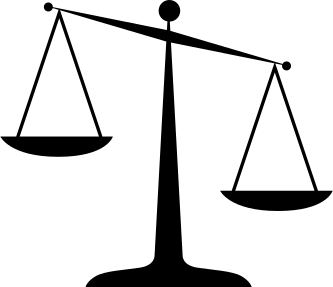
\includegraphics[width=0.23\textwidth]{pictures/scales.pdf}
  \vspace{-5mm}
  \end{center}
  \caption{Balance scales (illustrative image).}
  \vspace{-10mm}
\end{wrapfigure}

The problem of finding a counterfeit coin among regular coins in the fewest
  number of weighings on a pair of scales balance is the folklore of
  recreational mathematics.

In all problems of this kind, you can use the scales only to weight the coins.
You put some coins on the left pan, the same number of coins on the right pan
  and get one of the 3 possible outcomes.
Either both the sides weight the same (denoted ``='')
  or the left side is lighter (``<''),
  or the right side is lighter (``>'').

The standard, easiest variant can be formulated as follows.

\begin{problem}[The nine coin problem] \label{pr:coins9}
You are given $n >= 3$ (typically 9) coins, all expect one have the same weight.
The counterfeit coin is known to be lighter.
Determine the coin in the minimal number of weightings.
\end{problem}

This problem is very easy as one can use \emph{ternary search} algorithm.
In short, we divide the coins into thirds, put one third agains another
  on scales.
If both sides weight the same, the counterfeit coin must be in the last third,
  otherwise it must be in the lighter third.
In this way, the size of search space reduces by a factor of 3 in one weighting,
  which is clearly optimal.

In 1940s, a more complicated variant was introduced by Grossman\cite{coins-grossman1945}.

%whether the counterfeit coin is underweight or overweight
\begin{problem}[The Twelve Coin Problem] \label{pr:coins12}
You are given $n >= 3$ (typically 12) coins, exactly one of which is counterfeit,
  but it is not known if it is heavier or ligher.
Determine the unique coin and its weight relavite to others
  in the minimal number of weightings.
\end{problem}

\begin{figure}
\includegraphics[width=\textwidth]{pictures/coins12.pdf}
\caption{Decision tree for The Twelve Coin Problem. \\
Leaf $x$ means that the coin number $x$ is lighter, $\underline{x}$ means that
the coin number $x$ is heavier.}
\label{fig:coins12tree}
\end{figure}

The optimal solution for $n=12$ requires 3 weightings and one of the optimal
  strategies is shown in \autoref{fig:coins12tree} as a decision tree.

The research usually focuses on bounds on the maximal value of $n$
  for which the problem can be solved in $w$ weighings, for a given $w$.
Thus a solution of a problem is usually formulated as a theorem like the
  following one.

\begin{theorem}[Dyson, \cite{coins-dyson1946}]\label{th:coins12}
There exists a scheme that determines the counterfeit coin and
  its type in \autoref{pr:coins12} with $w$ weighings,
  if and only if
  \[ 3 <= n <=\frac{3^w - 3}{2}. \]
\end{theorem}

\begin{proof}
We show the main part of the original Dyson's proof\cite{coins-dyson1946}
  here because of its elegant combinatorial idea.
We show a scheme for $n = \frac{1}{2}(3^w - 3)$.

Let us number the coins from $1$ to $n$.
To a coin number $i$, we assing
  two labels from $\{0,1,2\}^w$ -- those corresponding the numbers
  $i$ and $3^w - 1 - i$ in ternary form.
Notice that all possible labels are used exactly once, except for $0^w, 1^w$
  and $2^w$, which were not assigned to any coin.
The labeling has the property that you can
  get one label of a coin from the other by substituing $0$ by $2$ and $2$ by $0$.

A label is called ``clockwise'' if the first change of digit in it is
the change from $0$ to $1$, from $1$ to $2$, or from $2$ to $0$.
Otherwise, it is called ``anticlockwise''.
Thanks to the property we mentioned, one of the labels of a coin is always
  clockwise and the other is anticlockwise.

Let $C(i, d)$ be a set of coins such that $i$-th symbol in
  its clockwise label is $d$.
Since a permutation changing $0$ to $1$, $1$ to $2$ and $2$ to $0$ transfers
  coins from $C(i,0)$ to $C(i,1)$,
        from $C(i,1)$ to $C(i,2)$ and
        from $C(i,2)$ to $C(i,0)$,
  all the sets $C(i, d)$ contain exactly $n/3$ coins.
Now, let $i$-th experiment be the weighing of the coins $C(i,0)$ agains $C(i, 2)$.
It remains to show that the experiments uniquely determine the counterfeit coin.
Let $a_i$ be 0, 1, or 2 if the result of $i$-th experiment is
  left side is lighter, both are the same, or right side is lighter, respectively.

If the counterfeit code is overweight, the $i$-th symbol of its clockwise label
  must be $a_i$. On the other hand, if it is underweight, the $i$-th symbol of
  its anticlockwise label must be $a_i$.
The solution of the problem is therefore the coin with the label $a_1a_2...a_w$
  and is heavier than others if and only if this label is clockwise.
\autoref{fig:coins12scheme} shows an example of the construction for $n = 12 = \frac{1}{2}(3^3 - 3)$.

The case $n < \frac{1}{2}(3^w - 3)$ can be done similarly with some modifications
  to the labelling.
However, the scheme makes use of a genuine coin that was discovered in the first
  weighing and, therefore the following experiments depend on the outcome of
  the first.
Finally, the prove that the coin cannot be detected if
  $n > \frac{1}{2}(3^w - 3)$ can be done using information theory.

\begin{figure}
\begin{center}
\includegraphics{pictures/coins12-th.pdf}
\end{center}
\caption{Demonstration of the ternary label construction for $n=12$.}
\label{fig:coins12scheme}
\end{figure}
\end{proof}

Naturally, the problem was generalized in various ways and
  studied by many authors.
In ``Coin-Weighing Problems''\cite{coins-cwproblems1995}, Guy and Nowakovski
  gave a great overview of the research in the area until 1990s
  with an extensive list of references.
We list the most interesting variants and generalizations below.

\begin{itemize}
\item \textbf{Weight of counterfeit coin.}
  Either it is known whether the counterfeit coin is lighter or heavier,
  or it is not.
  The first one allows for more generalizations due to its simpler nature
  but both problems have been heavily researched.
\item \textbf{Number of counterfeit coins.}
  In the most common case, there is exactly one counterfeit coin,
    which allows for natural generalizations.
  First, a variant of \autoref{pr:coins9} with 2 or 3 counterfeit coins
   was studied\cite{coins-2fakes}\cite{coins-3fakes},
  then with $m$ counterfeit coins in general\cite{coins-mfakes}.
  Some authors studied the problem for unknown number of counterfeit coins
  \cite{coins-unknownfakes},
  or for \emph{at most} $m$ counterfeit coins\cite{coins-atmostfakes}.
\item \textbf{Additional regular coin(s).}
  In some cases, it may help if you are given an additional coin (or more coins),
    which is guaranteed not to be counterfeit.
  For example, for $n = 13$ in \autoref{pr:coins12}, you need 4 weightings.
  However, if you are given this one extra coin, you can determine the
    solve in just 3 weightings\cite{coins-dyson1946}.
\item \textbf{Non-adaptive strategies.}
  In this popular variant of the problem you have to announce all experiments
    in advance and then just collect the result.
  In other words, later weighings must not depend on the outcomes of the earlier weighings.
  Notice that the scheme constructed in the proof of \autoref{th:coins12} for
  $n = \frac{1}{2}(3^w - w)$ is indeed non-adaptive.
  However, the original proof uses an adaptive scheme for a smaller $n$.
  This was later fixed, showing that there always exists an optimal scheme for
  \autoref{pr:coins12} which is non-adaptive\cite{coins-nonadaptive}.
\item \textbf{Unreliable balance.}
  This generalization introduces the possibility that
  one (or more) answers may be erroneous.
  The problem of errors/lies in general search problems is well studied,
    see \cite{games-lies}.
  It was applied on the counterfeit coin problem (\autoref{pr:coins9} variant)
  in \cite{coins-unreliable} with at most one erroneous outcome or in
  \cite{coins-unreliable} with two.
\item \textbf{Multi-arm balance.}
  In this variant, your balance has $k$ arms. You put the same number of coins
  on every arm and you get either the information that all
  weight the same or which arm is lighter or heavier
  than others\cite{coins-multiplearm}.
\item \textbf{Parallel weighting.}
  In this generalization, you have 2 (or $k$, in general)
    balance scales, you can weight different coins on
    the two scales simultaneously and it counts
    as only one experiment\cite{coins-parallel}.
  The motivation here is that the weighing takes some not insignificant time,
  you have more scales and strive to minimize the time the whole process takes.
\end{itemize}

%%%%%%%%%%%%%%%%%%%%%%%%%%%%%%%%%%%%%%%%%%%%%%%%%%%%%%%%%%%%%%%%%%%%%%%%%%%%%%%%
\section{Mastermind}

\begin{wrapfigure}{r}{0.32\textwidth}
  \begin{center}
  \vspace{-5mm}
  \includegraphics[width=0.28\textwidth]{pictures/mastermind.png}
  \vspace{-5mm}
  \end{center}
  \caption{Mastermind game (illustrative image).}
  \vspace{-10mm}
\end{wrapfigure}

\emph{Mastermind} is a classic 2-player board game invented
  by Mordecai Meirowitz in 1970[wiki].
The principle of the game is the same as of \emph{Bulls and Cows},
  it just uses colors instead of letters.

%%%%%%%%%%%%%%%%%%%%%%%%%%%%%%%%%%%%%%%%%%%%%%%%%%%%%%%%%%%%%%%%%%%%%%%%%%%%%%%%
\section{Other Problems and Applications}
\subsection{Black Box}
% obrazky
\subsection{Bags of Gold}
% obrazky

\subsection{Code 777}
% obrazky - kartičky set

\subsection{String matching}
% aplikace geno fenotyp

\subsection{Generalized Mastermind}
% aplikace - pin cracking



\chapter{General model}

\section{Notation and Terminology}
Let $\Form_\Var$ be the set of all prepositional formulas over
  the set of variables $\Var$;
  $\Val_\Var$ be the set of all valuations (boolean interpretation)
  of variables $\Var$.
Formulas $\form_0, \form_1 \in \Form_\Var$ are (semantically) equivalent,
  written $\form_0 \equiv \form_1$, if
  $\val(\form_0) = \val(\form_1)$ for all $\val\in\Val_\Var$.
We say that \emph{$\val$ is a model of $\form$}
  or that \emph{$\val$ satisfies $\form$}
  if $\val(\form) = 1$.

% In the whole text, we want to identify equivalent formulas.
% Therefore, let $\Form_\Var = \Form^*_\Var/\!\!\equiv$ and in the sequel,
%   let us identify a formula with its corresponding equivalence class.


For a formula $\form\in\Form_\Var$, let
  $\numval_\Var{\form} = |\{ \val\in\Val_\Var \| \val(\form) = 1 \}|$
  be the number of models of $\form$ (valuations satisfying $\form$).
%This definition is correct as equivalent formulas has same number of models.
We often omit the index $\Var$ if it is clear from the context.

% For any unary predicate $P$, $\#i\in A.P(i) = |\{ i\in A \| P(i)\}|$.
%   We often omit the ``$\in A$'' part and write only $\#i.P(i)$
%   if the range of $i$ is clear from the context.

The set of all permutations of a set $\Var$ (bijections $\Var->\Var$)
  is denoted by $\Perm_\Var$ and
  $\idperm_\Var$ is the identity permutation.

%-------------------------------------------------------------------------------
% DEF: CODE BREAKING GAME
\section{Formal definition}

Code breaking games are game between two players -- a \emph{codemaker}
  and a \emph{codebreaker}.
The codemaker selects a secret code and then evaluates the experiments
  performed by the codebreaker.
The codebreaker chooses and performs experiments and collects partial
  information about the code according to some rules.
The codebreaker strives to reveal the code in minimal number of experiments.
... (introduction)

Within the framework of propositional logic,
  we represent the secret code as a valuation
  of propositional variables.
The game can be represented as a \emph{set of variables},
  \emph{initial restriction} (a formula that is guaranteed to be satisfied),
  and a set of \emph{possible experiments}.
A finite set of possible \emph{outcomes} is associated with each experiment.
Outcome is a propositional formula that represents the partial information,
  which the codebreaker can gain from the experiment.

The number of experiments is typically very large
  (such as 36894 for the Counterfeit-coin Problem \ref{prob-coins})
  but most of them have same structure and yield similar outcomes.
Therefore we opt for a compact representation of an experiment as a pair
  (type of experiment, parametrization), where parametrization is a string
  over a defined alphabet.
This whole idea is formalized below.

\begin{definition}[Code Breaking Game] \label{def-game}
A \emph{Code Breaking Game} is a septuple
  $\game = (\Var, \init, \Expt, \Sigma, \Exp, F, \outcome)$, where
  \begin{itemize}
  \item $\Var$ is a finite set of propositional variables,
  \item $\init \in \Form_\Var$ is a satisfiable prepositional formula,
  \item $\Expt$ is a finite set of types of experiments,
  \item $\Sigma$ is a finite alphabet,
  \item $\Exp \subseteq \Expt \times \Sigma^\star$ is an \emph{experiment} relation,
  and
  \item $F$ is a finite collection of functions of type $\Sigma -> \Var$,
  \item $\outcome: \Expt -> 2^{\PForm_{\Var,F,\Sigma}}$ is an
  \emph{outcome function} such that $\outcome(\expt)$ is finite
  for any $\expt\in\Expt$. Definition of $\PForm$ follows (Definition \ref{def-pform}).
  \end{itemize}
\end{definition}

\begin{definition}[Parametrized formula] \label{def-pform}
A set of \emph{parametrized formulas} $\PForm_{\Var,F,\Sigma}$ is a set of
 all strings $\pform$ generated by the following grammar:
$$ \pform ::= x \| f(\$n) \| \pform \circ \pform \| \neg \pform,$$
where $x\in\Var$, $f\in F$, $n \in\Nset$, and $\circ\in\{\wedge, \vee, =>\}$.
By $\pform(\param)$ we denote application of a parametrization $\param\in\Sigma^\star$
on a formula $\pform$, which is defined recursively on the structure of $\pform$ in the following way:
\begin{align}
(x)(\param) &= x, \\
(f(\$n))(\param) &= f(\param[n]),\\
(\pform_1\circ\pform_2)(\param) &= \pform_1(\param) \circ \pform_2(\param),\\
(\neg\pform)(\param) &= \neg(\pform(\param)).
\end{align}
\end{definition}

We use the special symbol $\$$ in $f(\$n)$ so that $n$ cannot be mistaken for
  the argument of $f$, which is $n$-th symbol of the parametrization.
Note that if $f(\$n)$ apperas in $\pform$ and $|\param|<n$, then
  $\pform(\param)$ is undefined. \TODO{Or false? Does it matter? ...}

For the sake of simplicity, let us denote the set of possible outcomes for
  an experiment $\exp = (\expt, \param) \in \Exp$ by
  $\outcome(\exp) = \{ \pform(\param) \| \pform\in\outcome(\expt)\}$.

The compact representation with parametrized formulas does not restrict
  the class of games that can fit this definition.
If no two experiments
  can be united under the same type, every experiment can have its own type and
  allow only one possible parametrization.

\begin{definition}[Solving process]
An \emph{evaluated experiment} is a pair $(e, \form)$ such that $\form\in\outcome(e)$.
Let us denote the set of evaluated experiments by $\Omega$.

A \emph{solving process} is a finite or infinite sequence of evaluated experiments.
\end{definition}

For simplicity, we omit the brackets around the pairs and write
  \[
  \proc = \exp_1, \form_1, \exp_2, \form_2, ...
  \]
We use the notation $\proc(i) = \exp_i$ and $\proc[i] = \form_i$
  to refer to the $i$-th experiment and $i$-th formula, respectively.
For $k\in\Nseto$, $k <= |\proc|$ we denote by
  $\aknow{\proc}{k} = \form_0 \wedge \form_1 \wedge ... \wedge \form_k$
  the accrued knowledge after $k$ experiments.

\TODO{Update:} Let us now describe the course of the game in the defined terms.
First, the codemaker choose a valuation $\val$ of $\Var$
  which satisfies $\init$.
Then, the codebreaker successively chooses a type $\expt\in\Expt$ and
  a parametrization $\param\in\Sigma^*$ such that $(\expt, \param)\in\Exp$.
The codemaker gives the codebreaker a formula $\form\in\outcome((\expt, \param))$
  which is satisfied by the valuation $\val$.

Here we hit a problem -- so that the codemaker can always fulfill the last step,
  there must be a formula $\form\in\outcome(\exp)$ satisfied by any valuation.
Since it might make sense to allow multiple satisfied formulas, we restrict
  ourselves to game where the outcome is uniquely defined for given valuation.

\begin{definition}[Well-formed game] \label{def-wellformed}
A code-breaking game is \emph{well-formed} if for all $\exp \in \Exp$,
\begin{equation}
\forall\val\in\Val_\Var:
  \val(\init) = 1 ==> \exists \textrm{ exactly one }
     \form\in\outcome(\exp)\;.\; \val(\form) = 1
\end{equation}
\end{definition}

In sequel, we suppose a game to be well-formed, if not stated otherwise.
Note that this property is not easy to check.

%-------------------------------------------------------------------------------
% EXAMPLE: FAKE-COIN PROBLEM

\begin{example}[Fake-coin problem] \label{form-fake-coin1}
Fake-coin problem with $n$ coins, one of which is fake, can be formalized as
a code breaking game
$\mathcal{F}_n = (\Var, \init, \Expt, \Sigma, \Exp, F, \outcome)$.

\begin{itemize}
\item
$\Var = \{x_1, x_2, ..., x_n, y\}$, \\
$\init = \exactly{1}\{x_1, ..., x_n\}$. \\
Intuitively, variable $x_i$ tells weather the coin $i$ is fake.
Variable $y$ tells weather it is lighter or heavier.
Formula $\init$ says that exactly one coin is fake.

\item
$\Expt = \{ w_2, w_4, ..., w_n \}$, \\
$\Sigma = \{1, 2,...,n\}$, \\
$\Exp = \bigcup_{1<=m<=n/2} \{ (w_{2m}, \param) \|
  \param \in \{1,...,n\}^{2m}, \forall x\in\Var. \#_x(\param)<=1 \}. $\\
There are $n/2$ types of experiment -- according to the number of coins we put on the weights.
The alphabet contains natural numbers up to $n$ and
possible parametrizations for $w_{2m}$ are strings of length $2m$ with no repetitions.

\item
$F = \{ f_x \}$, where $f_x(i) = x_i$ for $1 <= i <= n$, \\
$\outcome(w_m) = $ \vspace{-3mm}
\begin{align*}
  \big\{
& ((f_x(\$1) \vee ... \vee f_x(\$m)) \wedge \neg y) \vee ((f_x(\$m+1) \vee ... \vee f_x(\$2m)) \wedge y), \\
& ((f_x(\$1) \vee ... \vee f_x(\$m)) \wedge y) \vee ((f_x(\$m+1) \vee ... \vee f_x(\$2m)) \wedge \neg y), \\
& \neg (f_x(\$1) \vee ... \vee f_x(\$2m)) \big\}.
\end{align*}
There are 3 possible outcomes of every experiment.
First, the right side is heavier. This happens if the fake coin is lighter and it appears in the first half of the parametrization, or if it is heavier and it appears in the second half. Second, analogously, the left side is heavier.
Third, the weights are balanced if the fake coin do not participate in the experiment.
\end{itemize}
\end{example}

%-------------------------------------------------------------------------------
% EXAMPLE: FAKE-COIN PROBLEM - alternative

\begin{example}[Fake-coin problem, alternative] \label{form-fake-coin2}
For demonstration purposes, here is another formalization of the same problem.
$\mathcal{F'}_n = (\Var, \init, \Expt, \Sigma, \Exp, F, \outcome)$.

\begin{itemize}
\item
$\Var = \{x_1, x_2, ..., x_n, y_1, y_2, ..., y_n\}$, \\
$\init = \exactly{1}\{x_1, ..., x_n, y_1, ..., y_n \}$. \\
Variable $x_i$ tells that the coin $i$ is lighter, variable $y_i$ tells that the coin $i$ is heavier.
Formule $\init$ says that exactly one coin is different.

\item
$\Expt, \Sigma, \Exp$ is defined as in Example \ref{form-fake-coin1}.

\item
$F = \{ f_x, f_y \}$, where $f_x(i) = x_i$ and $f_y(i) = y_i$ for $1 <= i <= n$, \vspace{-1.5mm}
\begin{flalign*}
\outcome(w_m) = \big\{ & (f_x(\$1) \vee ... \vee f_x(\$m)) \vee (f_y(\$m+1) \vee ... \vee f_y(\$2m)), & \\
& (f_y(\$1) \vee ... \vee f_y(\$m)) \vee (f_x(\$m+1) \vee ... \vee f_x(\$2m)), & \\
& \neg (f_x(\$1) \vee ... \vee f_x(\$2m) \vee f_y(\$1) \vee ... \vee f_y(\$2m)) \big\}. &
\end{flalign*}
\end{itemize}
\end{example}

%-------------------------------------------------------------------------------
% EXAMPLE: MASTERMIND

\begin{example}[Mastermind] \label{form-mastermind}
Mastermind puzzle with $n$ pegs and $m$ colors can be formalized as
a code breaking game
$\mathcal{M}_{n,m} = (\Var, \init, \Expt, \Sigma, \Exp, F, \outcome)$.

\begin{itemize}
\item
$\Var = \{x_{i,j} \| 1<=i<=n, 1<=j<=m \}$, \\
$\init = \bigwedge\left\{
  \exactly{1} \{x_{i,j} \| 1<=j<=m\} \| 1<=i<=n\right\}$. \\
Variable $x_{i,j}$ tells whether there is the color $j$ at position $i$.
Formula $\init$ says that there is exactly one color at each position.

\item
$\Expt = \{ g_{k_1,...,k_m} \| k_i \in \{1,...,n\}, \sum_ik_i = n \}$,\\
$\Sigma = C$, \\
$\Exp = \{(g_{k_1,...,k_m}, \param) \| \param\in\Sigma^{n}, \#i.(\param[i]=j)=k_j\}$.\\
The type $g_{k_1,...,k_m}$ covers all the guesses in which the number of $j$-colored pegs is $k_j$.
Therefore, two guesses for which we use the same pegs (pegs are just shuffled) are of the same type,
but if we change a peg for one with different color, it is other type of experiment.

\item
$F = \{ f_1, ..., f_n \}$, where $f_i(c) = x_{i,c}$ for $1<=i<=n$,
\vspace{-2mm}
\begin{flalign*}
\outcome(& g_{k_1,...,k_n}) =  \Big\{ &\\
 & \exactly{b}\{ f_i(\$i) \| 1<=i<=n \} \;\wedge &\\
 & \exactly{t}\bigcup
      \big\{
           \{ \atleast{l}(x_{1,j},...,x_{n,j}) \| 1 <= l <= k_j \}
           \| 1<=j<=m
      \big\} &\\
  &\hspace{2cm} \| 0<=b<=t, 0<=t<=n\Big\}.
\end{flalign*}
\TODO{Zdůvodnit proč to funguje.}
\end{itemize}
\end{example}

%-------------------------------------------------------------------------------
% EXAMPLE: MASTERMIND 2

\begin{example}[Mastermind (alternative)] \label{form-mastermind2}
$\mathcal{M'}_{n,m} = (\Var, \init, \Expt, \Sigma, \Exp, F, \outcome)$.

\begin{itemize}
\item
$\Var$ and $\init$ is defined as in Example \ref{form-mastermind}. \\

\item
$\Expt = \{ g \}$,\\
$\Sigma = C$, \\
$\Exp = \{(g, \param) \| \param\in\Sigma^{n}\}$.\\

\item
$F = \{ f_1, ..., f_n \}$, where $f_i(c) = x_{i,c}$ for $1<=i<=n$,
$\outcome(g) = \{ \textrm{Outcome}(b, w) \| 0<=b<=n, 0<=w<=n, b+w<=n \}$,
where $\textrm{Outcome}$ function is computed by the algorithm described below.
\end{itemize}

\newcommand{\BlackSymb}{\bullet}
\newcommand{\NoSymb}{\times}

Consider a fixed color combination (code) and a guess.
We assign a symbol $\BlackSymb$, $\NoSymb$ or a number to each position
  in the following way.
If the color at a position is same in the code and the guess, we assign
  $\BlackSymb$ to this position and the player gets a black peg for it.
If the color in the guess at position $i$ differs but it appears
  appears at position $j$ in the code, we assign $j$ to position $i$ and
  the player gets a white peg. Also, position $j$ must not be assigned
  $\BlackSymb$ and the number $j$ must not be assigned to any other position.
We assign $\NoSymb$ to all other positions.
For example, if the code is $1234$ and the guess is $5251$, the assignment is
 $\underline{\NoSymb\BlackSymb\NoSymb\:1}$.

We start the computation of Outcome$(b, w)$ with generation of
  all combinations of $\BlackSymb$, $\NoSymb$ and different numbers from $1$ to
  $n$,
  so that there is $b$-times $\BlackSymb$, $w$-times a number and
  no number refers to a position with $\BlackSymb$.

Next, for each combination, we generate a conjunction in the following way:
\begin{itemize}
\item For $\BlackSymb$ at position $i$, we add $f_i(\$i)$.
\item For a number $j$ at position $i$, we add $\neg f_i(\$i) \wedge f_j(\$i)$.
\item For $\NoSymb$ at position $i$, we add $\neg f_j(\$i)$ for any other position $j$ with $\NoSymb$.
\end{itemize}
The result is a disjunction of all these clauses, which effectively enumerates all the cases.

To get a better idea about the results, this is $\textrm{Outcome}(1, 1)$ for n = 4:

...
% \medskip
% \begin{scriptsize}$(
% \neg f_0(\$0) \wedge \neg f_1(\$1) \wedge \neg f_1(\$2) \wedge \neg f_2(\$1) \wedge \neg f_2(\$2) \wedge f_3(\$3)) \vee
% (\neg f_0(\$0) \wedge \neg f_0(\$1) \wedge \neg f_0(\$2) \wedge \neg f_1(\$0) \wedge \neg f_1(\$1) \wedge \neg f_2(\$1) \wedge \neg f_2(\$2) \wedge f_3(\$3)) \vee
% (\neg f_0(\$0) \wedge \neg f_0(\$1) \wedge \neg f_0(\$2) \wedge \neg f_1(\$1) \wedge \neg f_1(\$2) \wedge \neg f_2(\$0) \wedge \neg f_2(\$2) \wedge f_3(\$3)) \vee
% (\neg f_0(\$0) \wedge \neg f_0(\$2) \wedge \neg f_1(\$0) \wedge \neg f_1(\$1) \wedge \neg f_2(\$0) \wedge \neg f_2(\$1) \wedge \neg f_2(\$2) \wedge f_3(\$3)) \vee
% (\neg f_0(\$0) \wedge \neg f_0(\$1) \wedge \neg f_1(\$1) \wedge \neg f_1(\$2) \wedge \neg f_2(\$0) \wedge \neg f_2(\$1) \wedge \neg f_2(\$2) \wedge f_3(\$3)) \vee
% (\neg f_0(\$0) \wedge \neg f_0(\$1) \wedge \neg f_1(\$0) \wedge \neg f_1(\$1) \wedge \neg f_2(\$2) \wedge f_3(\$3)) \vee
% (\neg f_0(\$0) \wedge \neg f_0(\$1) \wedge \neg f_1(\$0) \wedge \neg f_1(\$1) \wedge \neg f_1(\$2) \wedge \neg f_2(\$0) \wedge \neg f_2(\$2) \wedge f_3(\$3)) \vee
% (\neg f_0(\$0) \wedge \neg f_0(\$2) \wedge \neg f_1(\$1) \wedge \neg f_2(\$0) \wedge \neg f_2(\$2) \wedge f_3(\$3)) \vee
% (\neg f_0(\$0) \wedge \neg f_0(\$2) \wedge \neg f_1(\$0) \wedge \neg f_1(\$1) \wedge \neg f_1(\$2) \wedge \neg f_2(\$1) \wedge \neg f_2(\$2) \wedge f_3(\$3)) \vee
% (\neg f_1(\$1) \wedge \neg f_1(\$3) \wedge \neg f_2(\$1) \wedge \neg f_2(\$2) \wedge \neg f_3(\$1) \wedge \neg f_3(\$2) \wedge \neg f_3(\$3) \wedge f_0(\$0)) \vee
% (\neg f_1(\$1) \wedge \neg f_1(\$2) \wedge \neg f_2(\$2) \wedge \neg f_2(\$3) \wedge \neg f_3(\$1) \wedge \neg f_3(\$2) \wedge \neg f_3(\$3) \wedge f_0(\$0)) \vee
% (\neg f_1(\$1) \wedge \neg f_1(\$2) \wedge \neg f_2(\$1) \wedge \neg f_2(\$2) \wedge \neg f_3(\$3) \wedge f_0(\$0)) \vee
% (\neg f_1(\$1) \wedge \neg f_1(\$2) \wedge \neg f_2(\$1) \wedge \neg f_2(\$2) \wedge \neg f_2(\$3) \wedge \neg f_3(\$1) \wedge \neg f_3(\$3) \wedge f_0(\$0)) \vee
% (\neg f_1(\$1) \wedge \neg f_1(\$3) \wedge \neg f_2(\$2) \wedge \neg f_3(\$1) \wedge \neg f_3(\$3) \wedge f_0(\$0)) \vee
% (\neg f_1(\$1) \wedge \neg f_1(\$3) \wedge \neg f_2(\$1) \wedge \neg f_2(\$2) \wedge \neg f_2(\$3) \wedge \neg f_3(\$2) \wedge \neg f_3(\$3) \wedge f_0(\$0)) \vee
% (\neg f_1(\$1) \wedge \neg f_2(\$2) \wedge \neg f_2(\$3) \wedge \neg f_3(\$2) \wedge \neg f_3(\$3) \wedge f_0(\$0)) \vee
% (\neg f_1(\$1) \wedge \neg f_1(\$2) \wedge \neg f_1(\$3) \wedge \neg f_2(\$1) \wedge \neg f_2(\$2) \wedge \neg f_3(\$2) \wedge \neg f_3(\$3) \wedge f_0(\$0)) \vee
% (\neg f_1(\$1) \wedge \neg f_1(\$2) \wedge \neg f_1(\$3) \wedge \neg f_2(\$2) \wedge \neg f_2(\$3) \wedge \neg f_3(\$1) \wedge \neg f_3(\$3) \wedge f_0(\$0)) \vee
% (\neg f_0(\$0) \wedge \neg f_0(\$3) \wedge \neg f_1(\$0) \wedge \neg f_1(\$1) \wedge \neg f_3(\$0) \wedge \neg f_3(\$1) \wedge \neg f_3(\$3) \wedge f_2(\$2)) \vee
% (\neg f_0(\$0) \wedge \neg f_0(\$1) \wedge \neg f_1(\$1) \wedge \neg f_1(\$3) \wedge \neg f_3(\$0) \wedge \neg f_3(\$1) \wedge \neg f_3(\$3) \wedge f_2(\$2)) \vee
% (\neg f_0(\$0) \wedge \neg f_0(\$1) \wedge \neg f_1(\$0) \wedge \neg f_1(\$1) \wedge \neg f_3(\$3) \wedge f_2(\$2)) \vee
% (\neg f_0(\$0) \wedge \neg f_1(\$1) \wedge \neg f_1(\$3) \wedge \neg f_3(\$1) \wedge \neg f_3(\$3) \wedge f_2(\$2)) \vee
% (\neg f_0(\$0) \wedge \neg f_0(\$1) \wedge \neg f_0(\$3) \wedge \neg f_1(\$0) \wedge \neg f_1(\$1) \wedge \neg f_3(\$1) \wedge \neg f_3(\$3) \wedge f_2(\$2)) \vee
% (\neg f_0(\$0) \wedge \neg f_0(\$1) \wedge \neg f_0(\$3) \wedge \neg f_1(\$1) \wedge \neg f_1(\$3) \wedge \neg f_3(\$0) \wedge \neg f_3(\$3) \wedge f_2(\$2)) \vee
% (\neg f_0(\$0) \wedge \neg f_0(\$1) \wedge \neg f_1(\$0) \wedge \neg f_1(\$1) \wedge \neg f_1(\$3) \wedge \neg f_3(\$0) \wedge \neg f_3(\$3) \wedge f_2(\$2)) \vee
% (\neg f_0(\$0) \wedge \neg f_0(\$3) \wedge \neg f_1(\$1) \wedge \neg f_3(\$0) \wedge \neg f_3(\$3) \wedge f_2(\$2)) \vee
% (\neg f_0(\$0) \wedge \neg f_0(\$3) \wedge \neg f_1(\$0) \wedge \neg f_1(\$1) \wedge \neg f_1(\$3) \wedge \neg f_3(\$1) \wedge \neg f_3(\$3) \wedge f_2(\$2)) \vee
% (\neg f_0(\$0) \wedge \neg f_0(\$3) \wedge \neg f_2(\$0) \wedge \neg f_2(\$2) \wedge \neg f_3(\$0) \wedge \neg f_3(\$2) \wedge \neg f_3(\$3) \wedge f_1(\$1)) \vee
% (\neg f_0(\$0) \wedge \neg f_0(\$2) \wedge \neg f_2(\$2) \wedge \neg f_2(\$3) \wedge \neg f_3(\$0) \wedge \neg f_3(\$2) \wedge \neg f_3(\$3) \wedge f_1(\$1)) \vee
% (\neg f_0(\$0) \wedge \neg f_0(\$2) \wedge \neg f_2(\$0) \wedge \neg f_2(\$2) \wedge \neg f_3(\$3) \wedge f_1(\$1)) \vee
% (\neg f_0(\$0) \wedge \neg f_2(\$2) \wedge \neg f_2(\$3) \wedge \neg f_3(\$2) \wedge \neg f_3(\$3) \wedge f_1(\$1)) \vee
% (\neg f_0(\$0) \wedge \neg f_0(\$2) \wedge \neg f_0(\$3) \wedge \neg f_2(\$0) \wedge \neg f_2(\$2) \wedge \neg f_3(\$2) \wedge \neg f_3(\$3) \wedge f_1(\$1)) \vee
% (\neg f_0(\$0) \wedge \neg f_0(\$2) \wedge \neg f_0(\$3) \wedge \neg f_2(\$2) \wedge \neg f_2(\$3) \wedge \neg f_3(\$0) \wedge \neg f_3(\$3) \wedge f_1(\$1)) \vee
% (\neg f_0(\$0) \wedge \neg f_0(\$2) \wedge \neg f_2(\$0) \wedge \neg f_2(\$2) \wedge \neg f_2(\$3) \wedge \neg f_3(\$0) \wedge \neg f_3(\$3) \wedge f_1(\$1)) \vee
% (\neg f_0(\$0) \wedge \neg f_0(\$3) \wedge \neg f_2(\$2) \wedge \neg f_3(\$0) \wedge \neg f_3(\$3) \wedge f_1(\$1)) \vee
% (\neg f_0(\$0) \wedge \neg f_0(\$3) \wedge \neg f_2(\$0) \wedge \neg f_2(\$2) \wedge \neg f_2(\$3) \wedge \neg f_3(\$2) \wedge \neg f_3(\$3) \wedge f_1(\$1)
% ).$
% \end{scriptsize} \medskip

However complicated this may look, note that it is not much different from
 the previous model where the complexity of the formulas was hidden in the
 Exactly and AtLeast macro operators.
\end{example}

We do not provide the formal definition of other Code breaking Games presented in
  Chapter \ref{ch-games}.
However, a computer language for game specification
  that is based on this formalism is introduced in Chapter \ref{ch-cobra}, and
  definition of all the games in this language can be found in Appendix \ref{app-games}.

%-------------------------------------------------------------------------------
% DEF: STRATEGY
\section{Strategies}

\begin{definition}[Strategy]
A \emph{strategy} is a function $\stg: \Omega^* -> \Exp$,
  determining the next experiment for a given finite solving process.
\end{definition}

A strategy $\stg$ together with a valuation $\val$ (satisfying $\form_0$)
  induce an infinite solving process
  \[
  \procstg{\stg}{\val} = \exp_1, \form_1, \exp_2, \form_2, ...,
  \]
  where
  $\exp_{i+1} = \stg(\exp_1, \form_1, ..., \exp_i, \form_i)$
  and
  $\form_{i+1} \in \outcome(\exp_{i+1})$
  is such that
  $\val(\form_{i+1}) = 1$,
  for all $i\in\Nset$.
Notice that due to the condition in Definition \ref{def-wellformed},
  there is always exactly one such $\form_{i+1}$.
We denote the knowledge accrued by $\stg$ on $\val$ after $k$ experiments
  by $\stgknow{\stg}{\val}{k}$.


We define \emph{length} of a strategy $\stg$ on a valuation $\val$,
  denoted $\stglen{\stg}{\val}$,
  as the smallest $k\in\Nseto$ such that
  $\stgknow{\stg}{\val}{k} = \form_0 \wedge \form_1 \wedge ... \wedge \form_k$ has only one model
  ($\numval_\Var{\stgknow{\stg}{\val}{k}} = 1$).
This corresponds to the point where we can uniquely
  determine the code.

Note that it always holds $\numval{\stgknow{\stg}{\val}{k}} > 0$
  because
  $\val(\form_i) = 1$ for all $i\in\Nseto$.

\TODO{Define average number of experiments.}

The \emph{worst-case number of experiments} $\lenmax{\stg}$
  of a strategy $\stg$ is the maximal length of the strategy on a valuation $\val$,
  over all models $\val$ of $\form_0$, i.e.
  \[
  \lenmax{\stg} = \max_{\val\in\Val_\Var, \;\val(\form_0) = 1} \stglen{\stg}{\val}.
  \]
We say that a strategy $\stg$ \emph{solves the game} if $\lenmax{\stg}$ is finite.
The game is \emph{solvable} if there exists a strategy that solves the game.

% \TODO{Není to jednoduchý, ale je to zajímavý?
% Given a code-breaking game $\game$, decide whether $\game$ is solvable.}

\begin{definition}[Optimal strategy]
A strategy $\stg$ is \emph{worst-case optimal} if
  $\lenmax{\stg} <= \lenmax{\stg'}$ for any strategy $\stg'$.
\end{definition}

\begin{lemma}
Let $b = \max_{\expt\in\Expt} |\outcome(\expt)|$ be the maximal number of
  possible outcomes of an experiment. Then for every strategy $\stg$,
  \[
  \lenmax{\stg} >= \lceil \log_b(\numval{\init}) \rceil.
  \]
\end{lemma}

\begin{proof}
For a fixed $\stg$ and $k = \lenmax{\stg}$,
  $\stgknow{\stg}{\val}{k}$ can \TODO{nabývat} at most
  $b^k$ values.
By pidgeon-hole principle, if $\numval{\init} > b^k$, there must be a valuation
  $v$ such that $\stgknow{\stg}{\val}{k} > 1$.
This would be a contradiction with $k = \lenmax{\stg}$ and, therefore,
  $\numval{\init} <= b^k$, which is equivalent with the statement of the lemma.
\end{proof}

\subsection{Non-adaptive strategies}
\begin{definition}[Non-adaptive strategy]
A strategy $\stg$ is \emph{non-adaptive} if it decides the next experiment
  based on the length of the solving process only, i.e.
  whenever
  $\proc_1 = e_1, \form_1, ..., e_k, \form_k$ and
  $\proc_2 = e'_1, \form'_1, ..., e'_k, \form'_k$,
  then $\stg(\proc_1) = \stg(\proc_2)$.

Non-adaptive strategies can be seen as functions $\Nseto -> \Exp$.
\end{definition}

Non-adaptive strategies corresponds to the well studied problems of
  static mastermind and
  non-adaptive strategies for the coutnerfeit coin problem.
We mention them here only to show the possibility of formulating these problems
  in our formalism but we do not study them any further.

\subsection{Memory-less strategies}

\begin{definition}[Memory-less strategy]
A strategy $\stg$ is \emph{memory-less} if it decides the next experiment
  based on the accumulated knowledge only, i.e.
  whenever
  $\proc_1 = e_1, \form_1, ..., e_k, \form_k$ and
  $\proc_2 = e'_1, \form'_1, ..., e'_l, \form'_l$
  are two solving processes such that
  $ \form_1 \wedge ... \wedge \form_k \equiv \form'_1 \wedge ... \wedge \form'_l$,
  then
  $\stg(\proc_1) = \stg(\proc_2)$.

Memory-less strategies can be considered as functions $\Form_\Var -> \Exp$.
\end{definition}

\begin{lemma}
Let $\stg$ be a memory-less strategy and $\val$ a model of $\init$.
If there exists $k\in\Nset$ such that
  $\numval{\stgknow{\stg}{\val}{k}} = \numval{\stgknow{\stg}{\val}{k+1}}$,
 then
  $\numval{\stgknow{\stg}{\val}{k}} = \numval{\stgknow{\stg}{\val}{k+l}}$
 for any $l\in\Nset$.
\end{lemma}

\begin{proof}
For the sake of simplicity, let $\know^k = \stgknow{\stg}{\val}{k}$.
There is a formula $\form\in\outcome(\know^k)$,
  such that $\know^{k+1} \equiv \know^{k} \wedge \form$.
Therefore, if $\know^{k+1}$ is satisfied by valuation $\val$, so must be $\know^{k}$.
Since $\numval{\know^{k}} = \numval{\know^{k+1}}$, the sets of
  valuations satisfying $\know^{k}$ and $\know^{k+1}$ are exactly the same
  and the formulas are thus equivalent.
This implies $\stg(\know^{k}) = \stg(\know^{k+1})$ and $\know^{k+2} \equiv \know^{k+1}\wedge \form \equiv \know^{k+1}$.

By induction,
  $\stg(\know^{k+l}) = \stg(\know^{k})$ and
  $\know^{k+l} \equiv \know^{k}$
  for any $l\in\Nset$.\qed
\end{proof}

\begin{definition}[Greedy strategy]
Let $f: \Form_\Var -> \Zset$.
A memory-less strategy $\stg$ is \emph{$f$-greedy} if
  for every $\form\in\Form_X$ and $\exp'\in\Exp$,
\[
\max_{\formx \in \outcome(\stg(\form)) \atop \SAT{\form\wedge\formx}} f(\form\wedge\formx) <=
\max_{\formx \in \outcome(e) \atop \SAT{\form\wedge\formx}} f(\form\wedge\formx).
\]
In words, a greedy strategy minimizes
  the value of $f$ on the formula in the next step.
We say $\stg$ is \emph{greedy} if it is $\numval_\Var{}$-greedy.
\end{definition}

\begin{lemma}
Let $b = \max_{\expt\in\Expt} |\outcome(\expt)|$ be the maximal number of
  possible outcomes of an experiment.
If for any \TODO{reachable} $\form\in\Form_\Var$,
\[
  \exists\exp . \max_{\formx\in\outcome(\exp)} \numval{(\form\wedge\formx)} =
  \left\lceil \frac{\numval{\form}}{b} \right\rceil,
\]
then a greedy strategy $\stg$ is optimal and
\[
  \lenmax{\stg} = \lceil \log_b(\numval{\init}) \rceil.
\]
\end{lemma}

\begin{example}
Greedy strategies are optimal in the fake-coin game $\mathcal{F}_n$.
\TODO{...}
\end{example}

% \begin{problem}
% Given a code-breaking game $\game$,
%   decide whether all greedy strategies are optimal.
% Hypothesis: It is the case for Fake-coin problem (?).
%   It is not the case for Mastermind[ref].
% \end{problem}

\section{Symmetries in code-breaking games}

The number of possible parametrizations of a type of experiment is typically very large,
  which makes the analysis a game much harder.
For example, consider the counterfeit-coin problem (\ref{prob-coins})
  and the experiment of weighting 4 coins against 4 coins.
There is $\frac{1}{2}\cdot {12 \choose 4}\cdot{8 \choose 4} = 17325$
 possible combinations for parametrization, but
 in the initial state (i.e. with no knowledge except for the initial restriction),
 all of them are equivalent -- they will give us the same information regardless of symmetries.

In this section, we formally define equivalence of two experiments
 and show that we can neglect all but one experiment in each equivalence class.
Further, we present several lemmas that will form the basis of
 our symmetry breaking algorithms in the Chapter \ref{chapter-cobra}.

\begin{definition}[Symmetric experiment]
For an experiment $\exp = (\expt, \param)$ and a permutation $\perm\in\Perm_\Var$,
  a $\perm$-symmetric experiment $\exp^\perm = (\expt, \param')\in\Exp$
  is an experiment of the same type such that
  $\{\form^\perm \in\outcome(\exp)\} = \{\form\in\outcome(\exp^\perm)\}$.
Clearly, no such experiment may exists.
\end{definition}

\begin{definition}[Symmetry group]
We define a \emph{symmetry group} $\symg$ as
  the maximal subset of $\Perm_\Var$ such that for
  every $\perm\in\symg$ and for every experiment $\exp\in\Exp$,
  there exists a $\perm$-symmetric experiment $\exp^\perm$.
\end{definition}

\begin{definition}[Consistent strategy]
A memory-less strategy $\stg$ is \emph{consistent} if and only if
  for every $\form\in\Form_\Var$ and every $\perm\in\symg$, there
  exists $\permx\in\symg$ such that $\form^\perm \equiv \form^\permx$ and
  $\stg(\form^\permx) = \stg(\form)^\permx$.
\end{definition}

\TODO{Example, na kterém bude vidět, že jednoduchá definice nevyhovuje, protože můžu vzít symetrie $\form$ a dostanu, že to má dávat různé věci.}

\begin{lemma}
Let $\stg$ be a memory-less strategy.
There exists a consistent memory-less strategy $\stgx$ such that
  $\stglen{\stg}{\val} >= \stglen{\stgx}{\val}$
  for all $\val\in\Val_X$ satisfying $\init$.
\end{lemma}

\begin{proof}
Similar to the proof of Lemma \ref{lma-opt-memoryless}.
Let us choose any total order $\form_1, \form_2, ...$ of $\Form_\Var$ such that
if $\form_i$ implies $\form_j$, then $i <= j$.
We build a sequence of strategies $\stg_0, \stg_1, \stg_2, ...$ in the following way:
Let $\stg_0 = \stg$ and for $i > 0,$
\begin{equation}
\stg_i(\form) = \left\{
 \begin{array}{lll}
 \stg_{i-1}(\form) & \textrm{ if } \not\exists\perm\in\symg.\form^\perm\equiv\form_i \\
 \procstg{\stg_{i-1}}{\val_i}(k_i + 1) &
    \textrm{ if } \exists\perm\in\symg.\form^\perm\equiv\form_i\textrm{, where }
    (v_i, k_i) = \argmin_K \stglen{\stg_{i-1}}{v} - k,\\
    & \textrm{ and }
    K = \{(v, k)\in\Val\times\Nseto \| \exists\perm.\stgknow{\stg_{i-1}}{v}{k}^\perm\equiv\form_i\}.
    \vspace{-2.5ex}
 \end{array}
 \right.
 \vspace{2.5ex}
\end{equation}
We prove that $\stglen{\stg_{i}}{v} <= \stglen{\stg_{i-1}}{v}$.
If there is no $k$ and $\perm$ such that $\stgknow{\stg_i}{v}{k}^\perm\equiv\form_i$ then
  the processes $\procstg{\stg_i}{v}$ and $\procstg{\stg_{i-1}}{v}$ are the same.
If the is such $k$ and \TODO{...}.

The last strategy of the sequence is consistent and satisfies the
  condition in the lemma. \qed
\end{proof}

\begin{definition}[Experiment equivalence]
An experiment $\exp_1\in\Exp$ is equivalent to $\exp_2\in\Exp$ with respect to $\form$,
  written $\exp_1\expeq{\form}\exp_2$,
  if and only if there exists a permutation $\perm\in\symg$ such that
 $ \{ \form\wedge\formx \| \formx\in\outcome(\exp_1) \} \equiv
   \{ (\form\wedge\formx)^\perm \| \formx\in\outcome(\exp_2) \} $.
\end{definition}

\begin{theorem}
Let $\stg, \stgx$ be two consistent memory-less strategies, such that
$\stg(\form) \expeq{\form} \stgx(\form)$ for any $\form\in\Form_\Var$.
There is a bijection $f:\Val_\Var -> \Val_\Var$ such that
$\stglen{\stg}{\val} = \stglen{\stgx}{f(\val)}$.
\end{theorem}

\begin{proof}
First, we prove by induction for any $k\in\Nseto$,
  there is a permutation $\perm\in \symg$ such that
  $(\stgknow{\stg}{\val}{i})^\perm = \stgknow{\stgx}{\val^\perm}{i}$
  for all $i\in\Nseto$, $i<=k$.
For better readability, let
  $\know_k = \stgknow{\stg}{\val}{k}$ and
  $\knowx_{k, \perm} = \stgknow{\stgx}{\val^\perm}{k}$

For $k=0$, take $\perm = \idperm_\Var$.
Clearly, $\stgknow{\stg}{\val}{0} = \init = \stgknow{\stgx}{\val^\idperm}{0}$.

For the induction step, suppose we have $\perm\in\symg$ such that
  $\know_i^\perm = \knowx_{i, \perm}$ for $i <= k$.
Further, suppose $\perm$ is such that
  $\stg(\know_k^\perm) = \stg(\know_k)^\perm$. \TODO{Víc zdůvodnit.}

Let $e_1 = \stg(\know_k)$, $e_2 = \stgx(\knowx_{k, \perm})$
  be the $(k+1)$-th experiments  of the strategies.
It holds
\begin{equation}
e_2 = \stgx(\knowx_{k, \perm})
    \expeq{\knowx_{k, \perm}}  \stg(\knowx_{k, \perm})
    \stackrel{IH}{=} \stg(\know_k^\perm)
    = \stg(\know_k)^\perm
    = e_1^\perm \label{eq:expsym}\tag{$\sim$}
\end{equation}

and, therefore, there exists $\permx\in\symg$ such that
\begin{align}
 \{ \knowx_{k, \perm} \wedge \formx \| \formx\in\outcome(\exp_2) \} &= %\stackrel{(\refeq{eq:expsym})}{=}
 \{ (\knowx_{k, \perm} \wedge \formx)^\permx \| \formx\in\outcome(\exp_1^\perm) \} = \label{eq:sets}\tag{*}\\
&= \{ (\know_k^\perm \wedge \formx^\perm)^\permx \| \formx\in\outcome(\exp_1) \} =
 \{ (\know_k \wedge \formx)^{\permx\perm} \| \formx\in\outcome(\exp_1) \}
\end{align}
As $\permx\in\symg$ and $\symg$ is a permutation group, $\permx\perm\in\symg$.

Since the game is well-formed,
  $v$ satisfies exactly one formula in
  $\{ \know_k \wedge \formx \| \formx\in\outcome(\exp_1) \}$.
Therefore $v^{\permx\perm}$ satisfies exactly one formula
  in
  $\{ (\know_k \wedge \formx)^{\permx\perm} \| \formx\in\outcome(\exp_1) \}  =
   \{ \knowx_{k, \perm} \wedge \formx \| \formx\in\outcome(\exp_2) \}$,
  which means that $v^{\permx\perm}$ satisfies $\knowx_{k, \perm}$.
\TODO{Tohle nefugujeee!}
From Lemma \ref{lma-accruedknowledge},
  $\knowx_{k, \perm} = \knowx_{k, \permx\perm}$.
Both $\know_{k+1}^{\permx\perm}$ and $\knowx_{k+1, \permx\perm}$ is thus the only
  formula from (\refeq{eq:sets}) satisfied by $v^{\permx\perm}$ and, therefore,
  $\know_{k+1}^{\permx\perm} = \knowx_{k+1, \permx\perm}$.



Now for a fixed $\val$, take $k = \stglen{\stg}{\val}$, take
  $\perm\in\symg$ such that
  $(\stgknow{\stg}{\val}{k})^\perm = \stgknow{\stgx}{\val^\perm}{k}$
  and define $f(\val) = \val^\perm$.
Since
 $(\stgknow{\stg}{\val}{i})^\perm = \stgknow{\stgx}{f(\val)}{i}$
 for $i <= k$
 and variable permutation preserves the number of models of a formula, i.e.
  $\numval{\form} = \numval{\form^\perm}$ for any
  $\form\in\Form_\Var$, $\perm\in\Perm_\Var$,
 we have
  $\stglen{\stg}{\val} = \stglen{\stgx}{f(\val)}$.
% \TODO{It remains to show that $f$ is a bijection.}
  % Suppose $f$ is not injective, and $f(\val_1) = f(\val_2)$.
  % By definition, the only model of
  \qed
\end{proof}

\begin{corollary}
Let $\stg_1, \stg_2$ be two consistent memory-less strategies, such that
  $\stg_1(\form) \expeq{\form} \stg_2(\form)$ for any $\form\in\Form_\Var$.
Then $\lenmax{\stg_1} = \lenmax{\stg_2}$
  and $\lenexp{\stg_1} = \lenexp{\stg_2}$.
\end{corollary}

For any accrued knowledge $\form$, this lemma gives us the right
to consider only one of the experiments
$\exp_1, \exp_2$ if $\exp_1 \sim_\form \exp_2$.

Now, we would love an algorithm that would, for a given formula $\form$,
generate a set of experiment, such that there is exaclty one expriment
from every equivalence class in $E/\sim_\form$.

% \TODO{...}

% For the following sections, let us fix an experiment type $t$.
% \subsection{Phase 1}

% \subsection{Phase 2}
\section{Symmetry Breaking}

% The number of possible parametrizations of a type of experiment is typically very large,
%   which makes the analysis a game much harder.
% For example, consider the conterfeit-coin problem (\ref{prob-coins})
%   and the experiment of weighting 4 coins against 4 coins.
% There is $\frac{1}{2}\cdot {12 \choose 4}\cdot{8 \choose 4} = 17325$
%  possible combinations for parametrization, but
%  in the initial state (i.e. with no knowledge except for the initial restriction),
%  all of them are equivelent -- they will give us the same information regardless of symmetries.

% In this section, we formally define equivalence of two experiments
%  and show that we can neglect all but one experiment in each equivelence class.
% Further, we present several lemmas that will form the basis of
%  our symmetry breaking algorithms in the Chapter \ref{chapter-cobra}.

%Since composition of permutations is a permutation, this is clearly an equivalence relation.
% \TODO{Tohle hrozně nefunguje. Musí být symetrické i experimenty.}
% Plán:
% \begin{itemize}
% \item zadefinovat symetrii množiny experimentů jako gropu permutací proměnných tak, aby $\forall e\in E \exists e^\pi$ (kde
% ).
% \item zadefinovat nějakou vlastnost hry (symetrická) - pokud pro nějaké $e$ existuje $e^\pi$, pak pro všechny
% \item říct, že pokud jsou parametrizace nějak normálně omezené (typicky libovolný řetězec, nebo řetězec bez opakování), tak je ta hra symetrická
% \item omezit se s analýzou jen na symetrické hry
% \item zadefinovat konzistentní strategii, jako strategii, která na zpermutovanou formuli zahraje zpermutovaný experiment
% \item zadefinovat ekvivalenci experimentů podle definice výše
% \item dokázat, že pokud mám strategie $\stg_1. \stg_2$ tak že $\stg_1(\form) \sim_\form \stg_2(\form)$,
% tak existuje permutace proměnných taková, že $|\procstg{\stg_1}{\val}| = |\procstg{\stg_2}{\val^\pi}|$
% \end{itemize}

\begin{definition}
For an experiment $\exp$ and a permutation $\perm\in\Perm_\Var$,
  a $\perm$-symmetric experiment $\exp^\perm\in\Exp$ is an experiment such that
  $\{\form^\perm \in\outcome(\exp)\} = \{\form\in\outcome(\exp^\perm)\}$.
Clearly, no experiment satisfying this may exists.
\end{definition}

\begin{definition}
A game $\game$ is \emph{symmetric} if it satifies the following implication:
If for an experiment $\exp$ exists a $\perm$-symmetric experiment $\exp^\perm\in\Exp$,
  then a $\perm$-symmetric experiment exists for every experiment.
\end{definition}

For the rest of this chapter, the game we analyze is \emph{symmetric}.

\begin{definition}
A memory-less strategy $\stg$ is \emph{consistent} if and only if
  $\stg(\form^\perm) = \stg(\form)^\perm$ for any $\form\in\Form_\Var$ and
  $\perm\in$ symmetry group of the set of experiments.
\end{definition}

\TODO{Aby mohla být strategie konzistentní, musí být hra symetrická.}

\newcommand{\expeq}[1]{\cong_{#1}}
\begin{definition}
An experiment $\exp_1\in\Exp$ is equivalent to $\exp_2\in\Exp$ with respect to $\form$,
  written $\exp_1\expeq{\form}\exp_2$,
  if and only if there exists a permutation $\perm\in\Perm_\Var$ such that
 $ \{ \form\wedge\formx \| \formx\in\outcome(\exp_1) \} \equiv
   \{ (\form\wedge\formx)^\perm \| \formx\in\outcome(\exp_2) \} $.
\end{definition}

\begin{lemma} \label{lma-accruedknowledge}
Let $\stg$ be a consistent memory-less strategy and let $\val_1$, $\val_2$ be two models of $\init$.
If $v_1$ is a model of $\stgknow{\stg}{\val_2}{k}$, then $\stgknow{\stg}{\val_1}{k} = \stgknow{\stg}{\val_2}{k}$.
\end{lemma}
\begin{proof}
Let $\proc_1 = \procstg{\stg}{\val_1}$, $\proc_2 = \procstg{\stg}{\val_2}$
and let $c <= k$ be the first place where $\proc_1$ and $\proc_2$ differs.
...
\end{proof}

\begin{theorem}
Let $\stg_1, \stg_2$ be two consistent memory-less strategies, such that
$\stg_1(\form) \expeq{\form} \stg_2(\form)$ for any $\form\in\Form_\Var$.
Then for any $k\in\Nseto$, there is a permutation $\perm\in Sym$ such that
$\perm\in Sym$ and $(\stgknow{\stg}{\val}{k})^\perm = \stgknow{\stgx}{\val^\perm}{k}$.
\end{theorem}

\begin{proof}
By Induction.

For simplicity, let
  $\know_k = \stgknow{\stg}{\val}{k}$ and
  $\knowx_{k, \perm} = \stgknow{\stgx}{\val^\perm}{k}$
For $k=0$ it clearly holds, as any \TODO{$\perm\in$ Sym(E) $\init = \init^\perm$.}

For the induction step, suppose $\know_k^\perm = \knowx_{k, \perm}$ and $\perm\in Sym$.
Let $e_1 = \stg(\know_k)$, $e_2 = \stgx(\knowx_{k, \perm})$. It holds
\[
e_2 = \stgx(\knowx_{k, \perm})
    \expeq{\knowx_{k, \perm}}   \stg(\knowx_{k, \perm})
    = \stg(\know_k^\perm)
    = \stg(\know_k)^\perm
    = e_1^\perm
\]

and, therefore, there exists $\permx\in Sym$ such that
\begin{align}
 \{ \knowx_{k, \perm} \wedge \formx \| \formx\in\outcome(\exp_2) \} &=
 \{ (\knowx_{k, \perm} \wedge \formx)^\permx \| \formx\in\outcome(\exp_1^\perm) \} = \label{eq:sets}\tag{*}\\
&= \{ (\know_k^\perm \wedge \formx^\perm)^\permx \| \formx\in\outcome(\exp_1) \} =
 \{ (\know_k \wedge \formx)^{\perm\permx} \| \formx\in\outcome(\exp_1) \}
\end{align}
As $\permx\in Sym(E)$ and $Sym$ is a permutation group, $\perm\permx\in Sym(E)$.

Since we suppose the game is well-formed (Definition \ref{def-wellformed}),
  $v$ satisfies exactly one formula in
  $\{ \know_k \wedge \formx \| \formx\in\outcome(\exp_1) \}$.
Therefore $v^{\perm\permx}$ satisfies exactly one formula
  in
  $\{ (\know_k \wedge \formx)^{\perm\permx} \| \formx\in\outcome(\exp_1) \}  =
   \{ \knowx_{k, \perm} \wedge \formx \| \formx\in\outcome(\exp_2) \}$,
  which means that $v^{\perm\permx}$ satisfies $\knowx_{k, \perm}$.
From Lemma \ref{lma-accruedknowledge}, $\knowx_{k, \perm} = \knowx_{k, \perm\permx}$.
Both $\know_{k+1}^{\perm\permx}$ and $\knowx_{k+1, \perm\permx}$ is thus the only
  formula from (\refeq{eq:sets}) satisfied by $v^{\perm\permx}$. \qed
\end{proof}

\begin{corollary}
Let $\stg_1, \stg_2$ be two consistent memory-less strategies, such that
$\stg_1(\form) \expeq{\form} \stg_2(\form)$ for any $\form\in\Form_\Var$.
Then $\lenmax{\stg_1} = \lenmax{\stg_2}$.
\end{corollary}

% For any accrued knowledge $\form$, this lemma gives us the right
% to consider only one of the experiments
% $\exp_1, \exp_2$ if $\exp_1 \sim_\form \exp_2$.

% Now, we would love an algorithm that would, for a given formula $\form$,
% generate a set of experiment, such that there is exaclty one expriment
% from every equivalence class in $E/\sim_\form$.
% \TODO{...}

% For the following sections, let us fix an experiment type $t$.
% \subsection{Phase 1}

% \subsection{Phase 2}

\chapter{COBRA tool}
\label{ch:cobra}
The main part of our work was development a general tool for analysis of
  code breaking games.
We named the tool COBRA, the COde-BReaking game Analyzer.
Currently, it can read a game specification given in a special language, which
  we describe first.
Then it can perform various tasks with the game, which are described in detail
  afterwards as \emph{modes of operation}.
In the end of this chapter, we describe the external tools and libraries COBRA uses,
  what we need them for, and some implementation details.
\TODO{.. odůvodnit volby které jsme udělali (...)}

The source code of the tool, together with detailed documentation
  and specification of the games described in \autoref{ch:games}
  can be found as an \TODO{electronic attachment} to this thesis.

The tool was developed under GitHub\footnote{\url{http://www.github.com}},
  so another way of obtaining the code is by cloning
  the git repository at \url{https://github.com/myreg/cobra}.
This website also serves as a homepage of the project, and contains
  all related documents.

COBRA is available under \emph{BSD 3-Clause License}\footnote{\url{http://opensource.org/licenses/BSD-3-Clause}},
  text of which is a part of the source codes.

\section{Input language}

\TODO{First we describe the low-level language that is the input of our COBRA tool. }

\subsection{Low-level language}

\newcommand{\symb}[1]{\;\textcolor{DarkBlue}{\textrm{$<$#1$>$}}\;}
\newcommand{\txt}[1]{\;\textcolor{DarkRed}{\textsc{#1}}\;}
\newcommand{\term}[1]{\;\textrm{#1}\;}
\begin{align*}
\symb{code} ::=\;& \symb{line} \| \symb{code} \symb{line}\\
\symb{line} ::=\;& \txt{Variable} \term{ident} \| \txt{Variables} \symb{ident-list} \| \\
  & \txt{Restriction} \symb{formula} \| \txt{Alphabet} \symb{string-list} \| \\
  & \txt{Mapping} \term{ident} \symb{ident-list} \| \txt{Experiment} \term{string} \term{int} \| \\
  & \txt{Params-distinct} \symb{int-list} \| \txt{Params-sorted} \symb{int-list} \| \\
  & \txt{Outcome} \term{string} \symb{formula} \\
\symb{formula} ::=\;&  \term{ident} \| \txt{(} \symb{formula} \txt{)} \| \txt{!} \symb{formula} \| \\
 & \symb{formula} \txt{and} \symb{formula} \| \symb{formula} \txt{or} \symb{formula} \| \\
 & \txt{And(} \symb{formula-list} \txt{)} \| \txt{Or(} \symb{formula-list} \txt{)} \| \\
 & \symb{formula} \txt{$\rightarrow$} \symb{formula} \| \symb{formula} \txt{$\leftarrow$} \symb{formula} \| \\
 & \symb{formula} \txt{$\leftrightarrow$} \symb{formula} \| \term{ident} \txt{(\$} \term{int} \txt{)} \| \\
 & \txt{AtLeast-} \term{int} \txt{(} \symb{formula-list} \txt{)} \| \\
 & \txt{AtMost-} \term{int} \txt{(} \symb{formula-list} \txt{)} \| \\
 & \txt{Exactly-} \term{int} \txt{(} \symb{formula-list} \txt{)} \\
\symb{ident-list} ::=\;& \term{ident} \| \symb{ident-list} \txt{,} \term{ident} \\
\symb{int-list} ::=\;& \term{int} \| \symb{int-list} \txt{,} \term{int} \\
\symb{formula-list} ::=\;& \symb{formula} \| \symb{formula-list} \txt{,} \symb{formula} \\
\symb{string-list} ::=\;& \term{string} \| \symb{string-list} \txt{,} \term{string}
\end{align*}

\subsection{Python preprocessing}
\TODO{Lepsi generovat, based on python with extra function calls.}
\TODO{example: MM}

%%%%%%%%%%%%%%%%%%%%%%%%%%%%%%%%%%%%%%%%%%%%%%%%%%%%%%%%%%%%%%%%%%%%%%%%%%%%%%%%
\section{Basic usage}
\TODO{Cobra vs cobra backend. Flagy, specifikace strategií - rozšířitelnost. Volba backendu, time overview. }

%%%%%%%%%%%%%%%%%%%%%%%%%%%%%%%%%%%%%%%%%%%%%%%%%%%%%%%%%%%%%%%%%%%%%%%%%%%%%%%%
\section{Modes of operation}

\subsection{Overview mode}

Prints masic statistics about the game and performes the well-formed check.
\TODO{How?}

\subsection{Simulation mode}
\TODO{Interactive vs one-step look ahead strategy.}

\subsection{Strategy analysis mode}
\begin{description}
\item[Min-num.]
\item[Min-exp.]
\item[Entropy.]
\item[Fixed.]
\item[Most-parts.]
\end{description}

\subsection{Optimal strategy mode}
\TODO{Bude?}



\section{Modularity and extensibility}

COBRA uses external tools for SAT solving and graph canonization.
Nowadays, many high-performance SAT solvers are available
  and multiple tools for graph canonization exists.
COBRA was developed so that other external tools with the same functionality
  can be easily integrated.
\autoref{fig:components} shows a component diagram.
\begin{figure}[h]
\includegraphics[width=\textwidth]{pictures/modularity.pdf}
\caption{Component diagram of COBRA.}
\label{fig:components}
\end{figure}

Detailed requirements on a SAT solver and
  on a graph canonization tool are listed in the next sections.

If you want to try another SAT solver, alter the algorithm for model counting,
  or test any other modification,
  you can implement your own solver class that inherits from \texttt{Solver} and
  implements all the necessary methods.

Check the \texttt{solver.h} file and the documentation therein
  for the information about the exact functions required.
Further, you need to to include the file with your class in
  \texttt{main.cpp} and add a new case
  into the \texttt{get\_solver} function in this file.


COBRA can be easily extended with a new strategy or heuristics to selects experiments.
All available strategies are implemented in \texttt{strategy.h/strategy.cpp} file.
If you want to add a new strategy, create a corresponding function in this file
  and add an entry about the strategy
  to the \texttt{breaker\_strategies} table in \texttt{strategy.h}.
A strategy function takes a list of experiments as the only argument
  and returns the index of the selected one.

If the strategy is one-step look-ahead,
  you can use a provided template with a corresponding lambda function.
We demonstrate this possibility with a code snippet of
  the exact implementation of the \emph{exp-models} strategy below.
For exact details, see the documentation in the file.

\begin{lstlisting}[language=C++]
uint breaker::exp_num(vec<Option>& options) {
  return minimize([](Option& o){
    auto models = o.GetNumOfModels();
    int sumsq = 0;
    for (uint i = 0; i < o.type().outcomes().size(); i++) {
      sumsq += models[i] * models[i];
    }
    return (double)sumsq / o.GetTotalNumOfModels();
  }, options);
}
\end{lstlisting}

\section{SAT solving} \label{s:cobra-sat}

COBRA uses a SAT solver for the following tasks.
\begin{itemize}
\item Compute the total number of possible codes.
\item Verify that an experiment is well-formed (see \autoref{s:cobra-modes} for details).
\item Identify satisfiable outcomes of an experiment and disregard the others.
\item Decide whether the game is finished -- whether the accumulated
  knowledge as a formula has only one model.
\item Evaluate the strategies -- count models, fixed variable, etc.
\end{itemize}

Most of these tasks require an \emph{incremental SAT solver}, i.e. a
  sat solver to which you can add constraints and take them back later.
Without this feature, we would have to call the solver from a clean state
  many times on the whole formula, which would ruin the computation time.

COBRA uses a SAT solver as an abstract class, which can have multiple implementations.
This allows a simple extension with another SAT backend.
The solver to be used can be specified with
  the \texttt{-b} or \texttt{--backend} switch.

Solver must implement the following methods:
\begin{itemize}
\item \textsc{AddConstraint}(formula). Adds a constraint to the SAT solver.
\item \textsc{Satisfiable()} $->$ Bool. Decides whether the current formula is satisfiable.
\item \textsc{GetAssignment()} $->$ Assignment.
  After \textsc{Satisfiable} call, this function retrieves
  a satisfying assignment from the solver.
\item \textsc{OpenContext(), CloseContext()}.
  This is our understanding of incremental SAT solving.
  \textsc{OpenContext} adds a context to a stack.
  Every call to \textsc{AddConstraint} adds the constraint to the current context.
  \textsc{CloseContext} removes all the constraint in the current context and removes it
  from the stack. It must be possible to nest contexts arbitrarily.
  The two methods are sometimes called just \textsc{Push} and \textsc{Pop}.
\item \textsc{HasOnlyOneModel()} $->$ Bool. Decides whether to formula has only one model.
  This can be implemented by asking whether the formula is satisfiable,
  if yes, retrieving the satisfying assignment, adding
  a clause with the assignment negated and asking for satisfiability again.
  Adding the new clause should be done in a new context in order not to pollute
  the solver state. The pseudocode is shown in \autoref{alg:onlyonemodel}.

\item \textsc{CountModels()} $->$ Int.
SAT solvers do not typically include support for model counting, the problem
  commonly referred to as \#SAT.
One solution is to use
  special tools designed for this purpose,
  such as SharpSAT\footnote{\url{https://sites.google.com/site/marcthurley/sharpsat}}
  \cite{sharpsat}.
However, these tools do not support incremental solving and
  must be run from a clean state for each formula models of which we want to count.

Second option is to use a SAT solver, repeatedly ask for satisfiability and
  add clauses that forbids the current assignment until we get
  an unsatisfiable formula. The pseudocode is shown in \autoref{alg:modelcounting2}.

Third option is to use a SAT solver and a simple backtracking approach,
  progressively assuming a variable to be true or false and cut the non-perspective
  branches.
The pseudocode is shown as a recursive function in \autoref{alg:modelcounting3}.
\end{itemize}

\begin{algorithm}[h]
\caption{Decision whether a formula has exactly one model.}
\label{alg:onlyonemodel}
\DontPrintSemicolon
\lIf{not \textsc{Satisfiable()}}{\Return{false}}
$v <- $ \textsc{GetAssignment()}\;
\textsc{OpenContext()}\;
\textsc{AddConstraint($\overline{x_1}\| ... \|\overline{x_n}$)},
  where $\overline{x_i}$ is $\neg\:x_i$ if $v(x_i) = 1$ and $x_i$ otherwise\;
$sat <- $\textsc{Satisfiable()}\;
\textsc{CloseContext()}\;
\Return{$\neg sat$}
\end{algorithm}
\begin{algorithm}[h]
\caption{Model counting, second option.}
\label{alg:modelcounting2}
\DontPrintSemicolon
$models <- 0$\;
\textsc{OpenContext()}\;
\While{\textsc{Satisfiable()}} {
  $v <- $ \textsc{GetAssignment()}\;
  \textsc{AddConstraint($\overline{x_1}\| ... \|\overline{x_n}$)},
    where $\overline{x_i}$ is $\neg\:x_i$ if $v(x_i) = 1$ and $x_i$ otherwise\;
  $models <- models + 1$\;
}
\textsc{CloseContext()}\;
\Return{$models$}
\end{algorithm}
\begin{algorithm}[h!]
\caption{Model counting, third option.}
\label{alg:modelcounting3}
\DontPrintSemicolon
$models <- 0$\;
$x <- $ any variable from $vars$\;
\textsc{OpenContext()}\;
\textsc{AddConstraint}($x$)\;
\lIf{\textsc{Satifiable()}}{$models <- models \:+ $ \textsc{count}($vars\setminus \{x\}$)}
\textsc{CloseContext()}\;
\textsc{OpenContext()}\;
\textsc{AddConstraint}($\neg x$)\;
\lIf{\textsc{Satifiable()}}{$models <- models \:+ $ \textsc{count}($vars\setminus \{x\}$)}
\textsc{CloseContext()}\;
\Return{$models$}
\end{algorithm}

COBRA includes three solver implementations which we describe next.

\subsection{PicoSat}
Picosat\footnote{\url{http://fmv.jku.at/picosat/}} \cite{picosat} is a simple,
  extensible SAT solver, which supports incremental SAT solving exactly in the way
  we need.

Bindings to Picosat are implemented in \texttt{PicoSolver} class.
This class also implements model counting algorithm \ref{alg:modelcounting3}
 as Picosat does not support model counting itself.


\subsection{MiniSat}

Minisat\footnote{\url{http://minisat.se/}} \cite{minisat} is a minimalistic,
  extensible SAT solver that won several SAT competitions in the past.

Minisat does not support incremental SAT solving in the manner we described,
  but it supports assumptions.
You can assume arbitrary number of unit clauses
  (i.e. that a variable is true of false) and ask for satisfiability under
  those assumptions.

The behaviour we want can be simulated by assumptions in the following way.
For each context, we create a new variable, say $a$.
Then, instead of adding clauses $C_1, C_2, ..., C_n$ to the context,
  we add clauses $\{\neg a, C_1\}$, $\{\neg a, C_2\}$, ... $\{\neg a, C_n\}$ and ask
  for satisfiability under the assumption $a$ (in general,
  assumption that all variables of open contexts are true).
Afterwards, when a context is closed, we add a unit clause $\{\neg a\}$,
  which effectively removes all the clauses added in the context.
The only minor issue with this approach is that the variable $a$ is wasted,
  the solver will remember it somewhere and may consume more memory.

Bindings to Minisat are implemented in \texttt{MiniSolver} class.
This class implements the context opening and closing in the way described above
and also model counting algorithm \ref{alg:modelcounting3}.

\subsection{Simple solver}

We include a special SAT solver, called \texttt{SimpleSolver} to show that
  the usage of a proper SAT solver in this application is justifiable.
Simple solver uses another SAT backend (Picosat) to generate all
  models of the initial constraint $\init$ (or of the first constraint, in general).
Later satisfiability questions with additional constraint are
  resolved by going though all possible codes (assignments) and
  checking that the constraints are satisfied.
Model counting and the other functions are implemented similarly.

\subsection{Transformation to CNF}

The input formula for a SAT solver must be typically specified
  in the conjunctive normal form(CNF).
As we do not have such requirement for formulas in the input format,
  and allow non-standard numerical operators,
  we need to transform a formula to CNF first.

The standard transformation works as follows.
First, we express the formula in a form
  that uses only negations, conjunctions and disjunctions as operators.
Then, we transform it to \emph{negation normal form} using De Morgan's laws
  and, finally, we use distributivity of conjunction and disjunction to
  move all the conjunction to the top level.
However, this may lead to an exponential explosion of the formula, so
another solution, called \emph{Tseitin Transformation}, is commonly used
  when converting a formula for a SAT solver\cite{tseitin}.

Imagine the formula as a circuit with gates corresponding to the logical operators.
Input vectors correspond to variable assignments and the circuit output
  is true if and only if the input assignment satisfies the formula.

For each gate, a new variable representing its output is created.
The resulting formula is a conjunction of sub-formulas that enforce
  the proper operation of the gates.

For example, consider an AND gate, inputs of which corresponds to variables
  $x$, $y$ and output corresponds to a variable $w$.
We need to ensure that $w$ is true if and only if both $x$ and $y$ are true,
  which is done by adding a sub-formula $w <-> (x \wedge y)$, which can be
  expressed in CNF as
\[
(\neg x \vee \neg y \vee w) \wedge
(x \vee \neg w) \wedge
(y \vee \neg w).
\]

Other gates types are handled similarly and this is done for all gates in the circuit.
Finally, the variables
  corresponding to the result of the top level operator is added
  to the resulting formula as a unit clause.

It remains to explain how we handle the numerical operators
  $\atleast$, $\atmost$ and $\exactly$.
We show it on the $\exactlyk{k}(f_1, ..., f_n)$ operator,
  others are transformed similarly. For simplicity,
  assume $f_i$ are variables; if not, we take the variable corresponding the
  the sub-formulas.

For each $l\in\{0,1,...,k\}$ and $m\in\{1,...,n\}$, $l <= m$, we create
  a new variable $z_{l,\:m}$ which will be true if and only if
  the formula $\exactlyk{l}(f_1, ..., f_m)$ is satisfied.
To enforce this assignment, we add sub-formulas of the form
  \[ z_{l,\:m} <-> (f_m \wedge z_{l-1,\:m-1}) \vee (\neg f_m \wedge z_{l,\:m-1}) \]
  for each $l > 1$, $m > 1$ (in CNF form, of course).
Special cases $l = m$ and $l = 0$ are equivalent to AND and OR formulas, respectively,
  and are handled accordingly.

The size of the resulting sub-formula is linear in $n\cdot k$.
Although this is not polynomial in the size of the input
  (supposing $k$ is encoded in binary form) but it is much better
  than the na\"ive solution to express the formula
  as a conjunction of the $n\choose k$ possibilities,
  which would be double exponential.

\section{Graph isomorphism}

To implement the suggested algorithm for detection of equivalent experiments,
  we need to solve the graph isomorphism problem, i.e. decide whether
  two given graphs are isomorphic.
Note that this problem is famous for not being proven either P-complete or
  NP-complete.
Although no polynomial algorithm for the problem is known,
  software tools are available for graph canonization problem,
  which are quite efficient for sparse graphs and can be used to
  decide graph isomorphism by comparison of canonical forms of the graphs.

Nauty\footnote{\url{http://pallini.di.uniroma1.it}}\cite{nauty} and
  Bliss\footnote{\url{http://www.tcs.hut.fi/software/bliss}}\cite{bliss}
  are programs primarily designed to compute automorphism groups of graphs
  but can produce a canonical labelling of the graph as well.
For various reasons including simple integration, we decided to choose Bliss.
For comparison of Nauty and Bliss,
  read an overview of the algorithms used by these tools in \cite{nautyblissoverview}
  and see benchmarks on the Nauty's website.

\section{Implementation details}

\subsection{Programming Language and Style}

Since the problems we solve are computationally very demanding,
  we had to choose a high-performing programming language.
The external tools we use, especially SAT solvers, are typically written in C/C++,
  so C++ was a natural choice for our tool.
COBRA is written in the latest standard of ISO C++, C++11, which
  contains significant changes both in the language and in the standard libraries
  and, in our opinion, improves readability and programmer's efficiency
  compared to previous versions.

We wanted the style of our code to be consistent and to use
  the language in the best manner possible according to industrial practice.
From the wide range of style guides available online
 we chose \emph{Google C++ Style Guide}\cite{googlestyle} and made
 the code compliant with all its rules except for a few exception.
The only significant violation are lambda functions, which are forbidden
due to various reasons,
 but we think they are more beneficial than harmful in this project.

\subsection{Requirements}
As noted earlier, compilation of COBRA requires a compiler,
  which supports all the C++11 features we use.
We recommend using standard \texttt{gcc} version $4.8$ or higher, or
 \texttt{clang} version $3.2$ or higher.

The tool is platform independent.
  We have tested compilation and functionality on
  on Linux (Ubuntu 14.04) and Mac OS X (10.9).

\subsection{Unit testing}
Unit testing has became a common part of software development process
  in the recent years.
Correctness is automatically a top priority for a tool of this kind and
  unit tests are a perfect way to capture potential programmer's error
  as soon as possible and avoid regression.

Lots of unit tests framework for C++ are available.
We focused on simplicity, minimal amount of work needed to add new tests
  and good assertion support, and opted for
  \emph{Google Test}\footnote{\url{https://code.google.com/p/googletest/}}.

All available tests are compiled and executed if you run \texttt{make test}
  in the tool directory.
This should serve as a basic sanity test and we highly recommend
  doing this in case you make any changes in the code.

\subsection{Functional tests}
\TODO{Blah.}

\chapter{Experimental results} \label{ch:exp}
In this chapter, we present experimental results of our tool on several code-breaking games.
We compare running times of the tool on various tasks with different SAT solvers and
  evaluate presented one-step look-ahead strategies.

In the tables below, MM($n$,$m$) refers to Mastermind with $n$ pegs and $m$ colours,
CC($n$) refers to the counterfeit coin problem with $n$ coins,
BG($n$,$m$) refers to Bags of gold problem with $n$ bags and balance scale capacity $m$ and
SM($n$,$m$) refers to the Mastermind variant with black markers only, i.e.
  for each guess, the codebreaker gets the number of positions at which the code
  and the guess match.

\section{Performance}

All experiments have been run on Intel Core i7-3770 3.40GHz and COBRA was
compiled with \texttt{gcc} 4.8.2.
The symmetry breaking engine has been turned off for this section,
  so that the differences between SAT solvers become more apparent.

The numbers in the following tables are running times in seconds with
  respective SAT solvers.
The last column (``\# calls'') states the total number of calls to
  the SAT solver during the task.
Model counting and counting the number of fixed variables is considered one call.

\autoref{tbl:exp-sat-wellformed} lists running times of the well-formed check
  of several code-breaking games.
Naturally, proper SAT solvers are orders of magnitude faster than simple solver
as well-formed check is based on verification of unsatisfiability of
  a (relatively) large formula.

\begin{table}[h]
\begin{center}
\begin{tabular}{|l|c|c|c|c|} \hline
Game & Simple & Minisat & Picosat  & \# calls \\ \hline
MM(4,6) & 174 & \textbf{2.7} & 3.2 & 1,296 \\
MM(5,4) & 217 & \textbf{14.3} & 34.8 & 1,024 \\
BG(12,12) & 3,539 &  \textbf{0.5} & 1.1 & 271 \\\hline
\end{tabular}
\caption{Running times (in seconds) of the well-formed check.}
\label{tbl:exp-sat-wellformed}
\end{center}
\end{table}

The first two lines of \autoref{tbl:exp-sat-sim} show execution times of the
  first experiment selection in Mastermind with $4$ pegs and $6$ colours.
The last two lines of the table list running times of the simulation of
  respective strategies on EDEE code.

As can be seen from the numbers, evaluation of ``parts'' strategy is slightly
  faster with Minisat than with simple solver.
However, since our model counting algorithm implemented on top of Minisat and Picosat
  is naive and unoptimized, ``max-models'' strategy evaluation is significantly faster
  with simple solver.

\begin{table}[h]
\begin{center}
\begin{tabular}{|l|c|c|c|c|} \hline
Task & Simple & Minisat & Picosat & \# calls \\ \hline
Select first exp. (parts) & 3.9 & \textbf{2.6} & 523 & 17,108 \\
Select first exp. (max-models) & \textbf{9.3} & 45.3 & $>$ 5,000 & 3,145 \\
Simulate (parts on EDEE) & 10.5 & \textbf{7.9} & 749 & 92,644 \\
Simulate (max-models on EDEE) & \textbf{15.1} & 32.3 & 3,024 & 31,061 \\\hline
\end{tabular}
\caption{Running times (in seconds) of simulation and strategy evaluation on MM(4,6).}
\label{tbl:exp-sat-sim}
\end{center}
\end{table}

\autoref{tbl:exp-sat-analyse}
  shows running times of strategy analysis.
A clear winner in this case is the simple solver based on
  model enumeration,
  which is not unexpected.
On lower levels of the backtracking algorithm,
  the analysed formulas have only very few models and the
  overhead with calling a proper SAT solver is greater
  than the na\"ive approach of a simple solver.

The results also show that model counting is harder than satisfiability questions.
The difference is not that significant for simple solver
 but, as we have already mentioned, our model counting algorithm is much slower.
That is the reason why the analysis of ``max-models'' strategy takes Minisat and Picosat
  much more time than analysis of ``parts'' strategy.

To summarize the results of this section,
Picosat turned out to be very slow on instances of this size. Minisat proved to be
useful for strategy evaluation in the first rounds, when the number of possible
models of the formula is relatively large.
Simple solver is a clear winner for strategy analysis.

A question arises whether we can benefit from a hybrid approach of
  using a SAT solver in the first steps and
  switching to the simple solver when the number of possibilities shrinks.
This was, however, beyond the scope of this thesis.

\begin{table}
\begin{center}
\begin{tabular}{|l|l|c|c|c|c|} \hline
Game & Strategy& Simple & Minisat & Picosat & \# calls \\ \hline
MM(3,4) & parts & 0.1 & 0.4 & 13.5 & 13,769 \\
MM(3,4) & max-models & 0.1 & 2.1 & 179 & 9,349 \\
MM(3,4) & exp-fixed & 0.3 & 17.4 & 1,974 & 15,002 \\
MM(4,4) & parts & 6.9 & 237 & $>$ 5,000 & 260,144 \\
MM(4,4) & max-models & 5.0 & 1,126 & $>$ 5,000 & 188,828 \\
MM(4,4) & exp-fixed & 24 & $>$ 5,000 & $>$ 5,000 & 329,820 \\
CC(20) & parts & 0.1 & 0.3 & 12.8 & 7,718 \\
CC(20) & max-models & 0.2 & 28 & 3,161 & 12,117 \\
CC(20) & exp-fixed & 0.3 & 73 & $>$ 5,000 & 14,273 \\\hline
% Analyse parts & CC(30) &  6.87 & 237 & ? & 260,144 \\
% Analyse parts & CC(30) &  0.08 & 0.34 & 13.5 & 13,769 \\
% Analyse max-models & CC(30) & ? & ? & ? & ? \\
% Analyse max-models & CC() & ? & ? & ? & ? \\
\end{tabular}
\caption{Running times (in seconds) of strategy analysis.}
\label{tbl:exp-sat-analyse}
\end{center}
\end{table}


\section{One-step look-ahead strategies}

In this section, we compare performance of one-step look-ahead strategies
defined in \autoref{sec:oslas} on the counterfeit coin problem,
Mastermind, and Mastermind with black markers only.

\subsection{The counterfeit coin problem}

The average-case number of experiments performed by one-step look-ahead
  strategies in the counterfeit coin problem
  for the number of coins from 3 to 40 is shown in \autoref{fig:exp-cc}.

Notice that larger number of coins does not necessarily mean that
  identifying the counterfeit coin is more difficult.
For example, the ``max-models'' strategy needs
  3.44 experiments on average to identify the counterfeit coin
  among 16 coins but only 3.41 if the number of coins is 17.
That is because the additional coin changes
  the number of models of some outcomes,
  which may lead to better experiment selection.

Interestingly, ``exp-fixed'' strategy outperforms all others
  on 20, 21, 23, 25 and 27 coins, while it seems to be
  generally worse.
Strategies ``parts'' and ``min-fixed'' are clearly unsuitable for
  a problem of this kind.

\begin{figure}[h]
\begin{center}
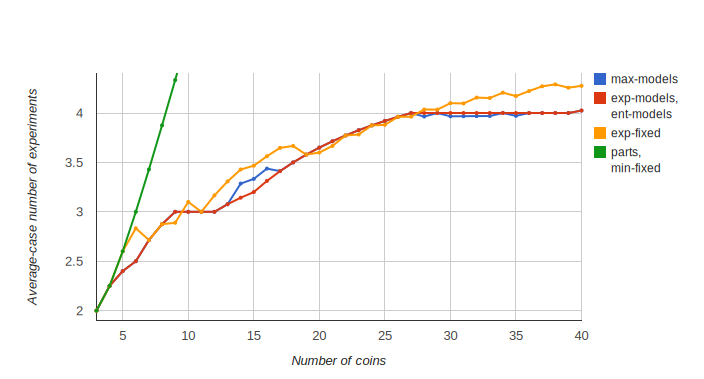
\includegraphics[width=\textwidth]{pictures/graph-cc.pdf}
\caption{Average-case number of experiments in the counterfeit coin problem.}
\label{fig:exp-cc}
\end{center}
\end{figure}

\subsection{Mastermind}

Results for Mastermind are shown in \autoref{tbl:exp-mm},
  rounded to three decimal places.
A clear winner in the average case is ``parts'' strategy,
  closely followed by ``max-models''.

In the worst case, ``max-models'' outperforms other
  strategies in all cases except MM(3,2).
This case was already mentioned in \TODO{..};
  the strategy needs four experiments due to an ``unlucky''
  choice of the first experiments.

Again, notice that larger size of the problem does not necessarily mean that
  revealing the secret is more difficult,
  as can be seen on the values for MM(5,2) and MM(5,3).

\begin{table}[h]
\begin{center}
\begin{tabular}{|c|c|c|c|c|c|c|c|c|c|c|c|c|}\hline
Game & \multicolumn{2}{c|}{max-mod} & \multicolumn{2}{c|}{parts}
& \multicolumn{2}{c|}{exp-mod} & \multicolumn{2}{c|}{ent-mod}
& \multicolumn{2}{c|}{min-fix} & \multicolumn{2}{c|}{exp-fix}\\ \hline
MM(2,3) & 2.667 & 4 & 2.333 & 3 & 2.444 & 3 & 2.444 & 3 & 2.667 & 4 & 2.444 & 3 \\
MM(2,6) & 3.667 & 5 & 3.667 & 5 & 3.861 & 5 & 3.861 & 5 & 4.611 & 7 & 4.167 & 6 \\\hline
MM(3,2) & 2.625 & 4 & 2.250 & 3 & 2.250 & 3 & 2.250 & 3 & 2.625 & 4 & 2.25 &  3 \\
MM(3,6) & 4.046 & 5 & 3.977 & 5 & 4.227 & 5 & 4.218 & 5 & 5.259 & 8 & 4.546 & 6 \\
MM(3,8) & 4.787 & 6 & 4.701 & 6 & 4.879 & 6 & 4.844 & 6 & 6.688 & 10 & 5.631 & 8 \\\hline
MM(4,2) & 2.750 & 4 & 2.750 & 4 & 3.063 & 4 & 3.063 & 4 & 3.250 & 5 & 3.063 & 4 \\
MM(4,6) & 4.476 & 5 & 4.374 & 6 & 4.626 & 6 & 4.643 & 6 & 5.765 & 9 & 5.231 & 7 \\
MM(4,7) & 4.837 & 6 & 4.743 & 6 & 4.962 & 6 & 4.947 & 6 & 6.476 & 10 & 5.945 & 8 \\
MM(4,8) & 5.183 & 6 & 5.102 & 7 & 5.293 & 7 & 5.272 & 7 & 7.213 & 11 & 6.410 & 9 \\\hline
MM(5,2) & 3.500 & 5 & 3.313 & 5 & 3.938 & 5 & 3.625 & 5 & 3.875 & 6 & 3.781 & 5 \\
MM(5,3) & 3.407 & 4 & 3.379 & 4 & 3.634 & 4 & 3.609 & 4 & 4.444 & 7 & 3.942 & 5 \\
MM(5,4) & 3.991 & 5 & 3.880 & 5 & 4.092 & 5 & 4.083 & 5 & 5.014 & 9 & 4.617 & 6 \\\hline
\end{tabular}
\caption{Average-case and worst-case number of experiments\\
  of one-step look-ahead strategies in Mastermind.}
\label{tbl:exp-mm}
\end{center}
\end{table}


\subsection{Mastermind with black markers only (string matching)}

Mastermind with black markers only is an example of a code-breaking game,
  where ``max-models'' does not perform so well.
Exact values rounded to two decimal points are shown in \autoref{tbl:exp-mmb}.

The best one-step look-ahead startegy for this game is ``ent-models'',
  the strategy based on the entropy of the number of models,
  closely followed by ``parts'' strategy.

\begin{table}[f]
\begin{center}
\begin{small}
\begin{tabular}{|c|c|c|c|c|c|c|c|c|c|c|c|c|}\hline
Game & \multicolumn{2}{c|}{max-mod} & \multicolumn{2}{c|}{parts}
& \multicolumn{2}{c|}{exp-mod} & \multicolumn{2}{c|}{ent-mod}
& \multicolumn{2}{c|}{min-fix} & \multicolumn{2}{c|}{exp-fix}\\ \hline
SM(3,3) & 3.15 &  4 &  2.89 & 4 & 2.89 & 4 & 2.89 & 4 & 3.52 &  4 & 3.52 &  4 \\
SM(3,6) & 6.1 &  8 &  5.58 & 7 & 5.74 & 8 & 5.53 & 7 & 8.3 & 13 &  8.28 &  13 \\
SM(3,12)& 10.76& 14 & 10.28 & 13& 10.5 & 14 & 10.23 & 13 &  17.41 & 31 &  13.3 &  22 \\ \hline
SM(6,3)& 4.94 &  6 &  4.5 & 7 & 4.5 & 6 & 4.47 &  6 & 6.5 & 7 & 6.16 &  7 \\
SM(6,6)& 8.61 & 12 &  8.2 & 12& 7.99 & 11 & 7.93 & 11 &  15.8 &  25 &  15.75 & 25 \\ \hline
\end{tabular}
\end{small}
\caption{Average-case and worst-case number of experiments
  of one-step look-ahead strategies \\ in Mastermind with black markers only.}
\label{tbl:exp-mmb}
\end{center}
\end{table}


\chapter{Conclusions}

We presented a general model of code-breaking games based on propositional logic,
  which can fit Mastermind, the counterfeit coin problem and many others.
Experiment equivalence was introduced and we proved that
  equivalent experiments can be disregarded during strategy analysis and
  optimal strategy synthesis.
We suggested an algorithm for equivalence
  testing based on graph isomorphism.

A computer language for code-breaking game specification was introduced
  and we developed a computer program that can perform various tasks
  with a given code-breaking game.
Using the tool, we reproduced some of the existing results for Mastermind,
  analysed other code-breaking games and
  evaluated strategies for experiment selection
  based on the number of fixed variables.

There are many more interesting things to try in this framework.
We present a few suggestions for future work in the next paragraphs.

First, our code-breaking game model can be further generalized in many ways.
Numerous possibilities arise if we allow experiments to have different costs.

Imagine Mastermind with another type of experiment
  that directly tells you a colour at a specified position.
What price must the new experiment have so that
  it is worth using it, given that the standard guess has unit cost?
%Another possibility is to limit the number of experiments of a type.

% Similarly, it may be interesting to limit
%   the number of experiments of a type.
% In the previous case, how would you play if you can
%   perform the new experiment only once?

Second, one-step look-ahead strategies provide us with
  a simple heuristics to select experiments.
However, if some experiments are assigned the same value, the
  lexicographically smaller experiment is chosen,
  which is not very reasonable.
% In fact, the ``parts'' strategy for Mastermind with 4 pegs and 6 colours
%   performs so well only due to a ``lucky'' choice in the first step.
% Experiments AABC and ABCD have both 14 satisfiable outcome
%   but the strategy chooses AABC because as it is lexicographically smaller.
\emph{Randomized strategies},
  where the experiment is selected from the experiments
  with the best value with uniform distribution
  may lead to many interesting results.

Third, look-ahead strategies can be naturally extended to more than one step.
This would lead to the \emph{minimax algorithm} applied to the tree of
  possible outcomes and experiments in the next rounds.
Evaluation of such strategies would be much more computationally demanding.
Would their performance be significantly better?

Finally, several completely different approaches for strategy synthesis
  were suggested for Mastermind.
In particular, genetic algorithms proved to be very useful for problems
  of larger sizes as they scale much better than the backtracking approach.
Can we apply these methods in our model?

For now, these interesting questions remain open.
We hope they will lead to further research in this area.


\pagestyle{plain}
%\printbibheading
\printbibliography
\clearpage
\addcontentsline{toc}{chapter}{Bibliography}

\chapter*{Contents of the electronic attachment}

An archive with source codes of Cobra
is available in the thesis repository in IS MU,
available online at \url{https://is.muni.cz/th/359972/fi_m/}.

The archive contains the following files and directories.

\bigskip
\begin{tabularx}{\textwidth}{lX}
 \texttt{examples/}\hfill & Directory with sample code-breaking game specifications,
        including Mastermind, the counterfeit coin problem and others. \\
\texttt{src/} & Directory with soures codes of Cobra. \\
\texttt{test/} & Directory with unit tests and functional tests. \\
\texttt{tools/} & Directory with source codes of external tools, Picosat release 957, Minisat version 2.2 and Bliss version 0.72. \\
\texttt{cobra} & The main executable. \\
\texttt{makefile} & Makefile with compilation rules and dependencies. \\
\texttt{LICENSE} & Full test of BSD License. \\
\texttt{README} & Short description of Cobra with basic information. \\
\end{tabularx}

%\clearpage
\addcontentsline{toc}{chapter}{Contents of the electronic attachment}

% \begin{appendices}
% \chapter{Specifications of sample games} \label{app:games}

Here we present specifications of the games defined in \autoref{ch:games}.
The language is described in \autoref{sec:lng}.


% \end{appendices}

% \printbibliography[keyword=cc,heading=subbibliography,title={Counterfeit Coin}]
% \printbibliography[keyword=mm,heading=subbibliography,title={Mastermind}]
% \printbibliography[keyword=other,heading=subbibliography,title={Other}]
\end{document}
